\documentclass[11pt]{article}  % required first line, though can vary;
                               % this says we will use 11-point font,
                               % in the "article" format
\usepackage{fancyhdr}
\usepackage{amsmath}
\usepackage{hyperref}
\usepackage{graphicx}
\usepackage{listings}
\usepackage[toc,page]{appendix}
\hypersetup{
colorlinks = true,
linkcolor = blue,
}
% material beginning with the percent sign is commentary, for human
% information purposes, not processed by the LaTeX system

% these \setlength etc. lines concern page layout, amount of paragraph
% indentation etc.; beginners should ignore them (but include them)
\setlength{\oddsidemargin}{0.0in}
\setlength{\evensidemargin}{0.0in}
\setlength{\topmargin}{0in}
\setlength{\headheight}{0in}
\setlength{\headsep}{0in}
\setlength{\textwidth}{6.5in}
\setlength{\textheight}{9.25in}
\setlength{\parindent}{15pt}
\setlength{\parskip}{2mm}

\title{\textbf{Final Project}}
\author{Tyler Welsh, Kim Dang, Anastasia Zimina}
\date{}
\renewcommand{\labelenumi}{\alph{enumi})}
%\renewcommand{\labelenumii}{\alph{enumii})}

%\pagestyle{fancy}
%\lhead{Tyler Welsh}
%\rhead{ID: 912341695}

\begin{document}  % required; the document starts here

\maketitle
\tableofcontents

\addcontentsline{toc}{section}{Problem A}
\newpage
\begin{center}
\section*{Problem A}
\end{center}

\indent The objective of this problem is to analyze the 100k Movie Lens data. We are interested in finding various confidence intervals, hypothesis tests, and linear regression models which will all be explained below. This data can be useful to confirm if there are any correlations between age and gender in regards to movie ratings, and see if there is any striking differences in the average movie ratings between men and women.\\
\indent Below is a list of explanations for various terms and phrases that will be used throughout the paper.
\begin{itemize}
    \item Confidence Intervals are useful for determining how 'certain' we are that a value falls into a certain range. In the following problems below, we will be using a 95\% confidence interval, which is saying, "We are 95\% sure the values fall within the given interval".
    
    \item Hypothesis tests help us determine whether certain claims, such as "The average ratings between men and woman are equal", are true or not.
    
    \item Linear Regression Models are ideal for estimating data given another set of data, such as "can we estimate the average rating of users dependent on their gender and age?".
    %KD: which sounds better: "regression models are ideal for..." or "regression models are great for..."?
        %T: Chose ideal
    \item Sample Size and Sample Population. The sample population is the total population of which we are sampling from, while the sample size is the size of our sample extracted from that population. 
    
    \item Sample Mean is the average value of the data we're interested in the given sample of data extracted from the sample population.
    
\end{itemize}
\indent The data set used for Problem A is a subset of the full Movie Lens 100k data, where we are generally only interested in the UserID, Age, Gender, and Rating. In most cases, Rating is reduced to the Average Mean Rating per User. All movie ratings are between 1 to 5 stars. The data can be viewed by running the mergeUserData() function (Appendix \ref{sec:probagen}) and viewing the output file "u.merged".

\indent Before we go through the various findings, it is important to note the difference in sample sizes. The number of men in the study is roughly triple the number of women in the study. This difference will have an affect on both the mean and standard deviation when finding differences of the means as well as the related confidence interval. The data found is still valid, but the intervals will generally be smaller with bigger sample sizes.
% in section 11.11 he mentions the importance of the sample size. I don't know where to put this, but the sample size of male movie ratings is almost three times as big as female. It affects both the mean and standard deviation and therefore, the difference of means, as well as the confidence interval. the confidence interval tend to be much smaller for bigger sample size. %

\begin{enumerate}
%USE 10.14 AND 10.20 we also use 11.6 for Hypo and 12.7 for regression as well as 12.11
\addcontentsline{toc}{subsection}{Confidence Interval for Mean Rating of Men}
%a
    \item An approximate 95\% confidence interval for the mean ratings by men is:
    \begin{align*}
        (3.556, 3.621) 
    \end{align*}
    This interval tells us that we are 95\% sure that the average male movie ratings fall between 3.556 and 3.621.
    
    There was a Sample Size of 670 Men, a Sample Mean of 3.588, and a Standard Deviation of 0.430
    %KD: we should put labels, like 670 people or ratings. otherwise these don't really make sense by themselves.
        %T: Will do
    
    The interval was found using the confIntMen() function in Appendix~\ref{sec:probaconf}.
    
\addcontentsline{toc}{subsection}{Confidence Interval for Mean Rating of Female}
%b
    \item An approximate 95\% confidence interval for the population mean rating by women is:
    \begin{align*}
        (3.530, 3.644)
    \end{align*}
    The interval found tells us that we are 95\% sure that the average movie ratings for women fall between the values 3.530 and 3.644.
    
    There was a Sample Size of 273 Women, a Sample Mean of 3.587, and a Standard Deviation of 0.481
    
    The interval was found using the confIntFemale() function in Appendix~\ref{sec:probaconf} 
    
\addcontentsline{toc}{subsection}{Confidence Interval for Mean Rating Difference Between Male and Female}
%c
    \item An approximate 95\% confidence interval for the difference between the two means in a) and b) is:
    \begin{align*}
        (-0.064, 0.067)
    \end{align*}
    This interval found tells us that we are 95\% sure that the difference between the average movie ratings between men and women is between -0.064 and 0.067. This is different than the previous intervals in that this interval doesn't give an average rating interval, but a difference in averages between two sets. When we have such a small interval, we can reason that the difference between the two networks is very small, and therefor not very significant. 
    % should we mention in the analysis that the difference is rather large for so small means? %
    % T: oh, in ch 10 or 11 he was talking about interpretation of significance tests: if we have really big means for 2 numbers, and then find the confidence interval for their difference, it is significant only iff  the interval is relatively large. something like that %
    
    There was a Sample Population of 670 Men and 273 Women, a Sample Mean of 3.588 for Male and 3.587 for Female, and a Standard Deviation of 0.430 for Male and 0.481 for Female.
    
    The interval was found using the confIntDiff() function in Appendix~\ref{sec:probaconf}
    
\addcontentsline{toc}{subsection}{Significance Testing for Population Mean Ratings}
%d
    \item The following is a significance test of the hypothesis that the male and female population means are equal. First we will go through the derivation and then evaluate the results.
    
    We want to test if $H_0 = c$ where $H_0$ is the Male mean ratings and $c$ is the Female mean ratings. We will use the equation:
    \begin{align*}
        Z = \frac{\bar{X} - c}{\sigma / \sqrt{n}}
    \end{align*}
    Where $\bar{X}$ is the sample mean ratings of men, $c$ is the female mean ratings,and $\sigma / \sqrt{n}$ is the standard error, with $sigma$ being the standard deviation of female mean ratings, and $n$ being the sample population of females.

    We will reject the hypothesis if the value of $Z$ is less than $-1.96$ or greater than $1.96$. This $1.96$ is generally called the 5\% level cutoff for hypothesis testing.
    
    Running the hypoth() function in~\ref{sec:probahypo} we found
    \begin{align*}
        Z = -0.086
    \end{align*}
    Since $Z$ lies within $-1.96$ and $1.96$, we do \textbf{NOT} reject the hypothesis that the male and female populations means are equal.

\addcontentsline{toc}{subsection}{Histograms of Mean Ratings}
%e
    \item Histogram plots for the average ratings of Men and Woman can be found on Page \pageref{fig:menhist}, where Figure~\ref{fig:menhist} is for the Men and Figure~\ref{fig:femalehist} is for the Women. From the graphs, we can see there is a large occurrence of mean ratings between 3.25 and 3.75  for Men and Women. What's interesting is that there are zero occurrences of 5 star ratings among men, but some for women.
    
    %T: TYLER FIX THE DAMN REFERENCES HISTO() IS NOT IN PROBACONF
    
    The histograms were created using the histo() function in Appendix~\ref{sec:probahisto}
    

\addcontentsline{toc}{subsection}{Confidence Interval for Mean Number of Ratings}
%f
    \item An approximate 95\% confidence interval for the difference between the number of ratings between men and women is:
    \begin{align*}
        (48,505.93, 48,534.07)
    \end{align*}
    This interval shows that the difference in the number of ratings of Men and the number of ratings of Women falls between 48,505.93 and 48,534.07. At first, this seems like an unusually high interval, but the provided data supports the results:

    Men had a mean number of ratings of 74260 while women had a mean number of ratings of 25740\\

    Now we can see why the interval is so large.
    
    We must stress that the number of ratings by male and female users are independent of each other. This is an important distinction that was left out earlier, but when calculating confidence intervals, the data must be independent for our mathematical work to hold. In previous problems, the mean rating of users have been independent, while the rating per movie was not independent. Because we are not working with actual rating values but the number of ratings per user in this situation, we need not worry about accounting for dependent variables.
    %KD: Tried to make it more formal. needs feedback.
    
    The interval was found using the confIntPopRat() function in Appendix~\ref{sec:probaconf}
    
\addcontentsline{toc}{subsection}{Confidence Interval for Population Proportion of Men}
%g
    \item An approximate 95\% confidence interval for the proportion of users who are male is:
    (0.683, 0.739)\\
   Instead of a raw numeric value like previous intervals, this confidence interval shows us a percentage value. This is the percentage of the users who are male, which is somewhere between 68.3\% and 73.9\%.
    
    The interval was found using the confIntPropMale() function in Appendix~\ref{sec:probaconf}

\addcontentsline{toc}{subsection}{Linear Modeling and Population Regression}
%h
    \item Here, we will use a Linear Regression Model to fit the data into a suitable model and make various calculations such as estimations of data given other data. For this problem, we will fit the MovieLens data into a linear function to predict a movie's rating based on a user's age and gender. The function we have produced is:
    \begin{align*}
        m_{W;H}(t) = \beta_0 + \beta_1 t_1 + \beta_2 t_2
    \end{align*}
    Which translates to:
    \begin{align*}
        \text{mean rating} &= \beta_0 + \beta_1\ \text{age} + \beta_2\ \text{gender}
    \end{align*}
    The $\beta$ values come from our data set: $\beta_0$ as our y-intercept using the Mean Rating data, $beta_1$ as part of our slope using the Age data, and $\beta_2$ as the other part of our slope using the Gender data.
    
    Below we can see the data produced by running the linear model function lm(). To see the full code used, see Appendix~\ref{sec:probalin}. We are only really interested in the Estimate and Std. Error columns of the (Intercept), A\$Gen, and A\$Age rows
    \begin{lstlisting}[basicstyle=\small]
    Call:
    lm(formula = A$Mean ~ A$Gen + A$Age)
    
    Residuals:
         Min       1Q   Median       3Q      Max 
    -2.06903 -0.25972  0.03078  0.27967  1.34615 
    
    Coefficients:
                 Estimate Std. Error t value Pr(>|t|)    
    (Intercept) 3.4725821  0.0482655  71.947  < 2e-16 ***
    A$Gen       0.0002862  0.0318670   0.009  0.99284    
    A$Age       0.0033891  0.0011860   2.858  0.00436 ** 
    ---
    Signif. codes:  0 '***' 0.001 '**' 0.01 '*' 0.05 '.' 0.1 ' ' 1

    Residual standard error: 0.4438 on 940 degrees of freedom
    Multiple R-squared:  0.008615,	Adjusted R-squared:  0.006505 
    F-statistic: 4.084 on 2 and 940 DF,  p-value: 0.01714
    \end{lstlisting}
    % i am not sure, but it might be worth mentioning that linear regression is a very poor representation of the data. With R-squared that small, it only explains about 8% of the data 
    Using this data, we can form a 95\% confidence interval for the estimation of mean rating from age and gender:
    \begin{align*}
        (3.375, 3.565)
    \end{align*}
    From this, we can say that the estimate mean rating from age and gender will fall somewhere between 3.375 and 3.565, which is not far off of previous data found. Figure~\ref{fig:regres} on page~\pageref{fig:regres} may also be useful to view for a visualization of the data.
    
    \begin{figure}[h]
    \centering
    \caption{The estimation of Mean Rating based on Age and Gender}
    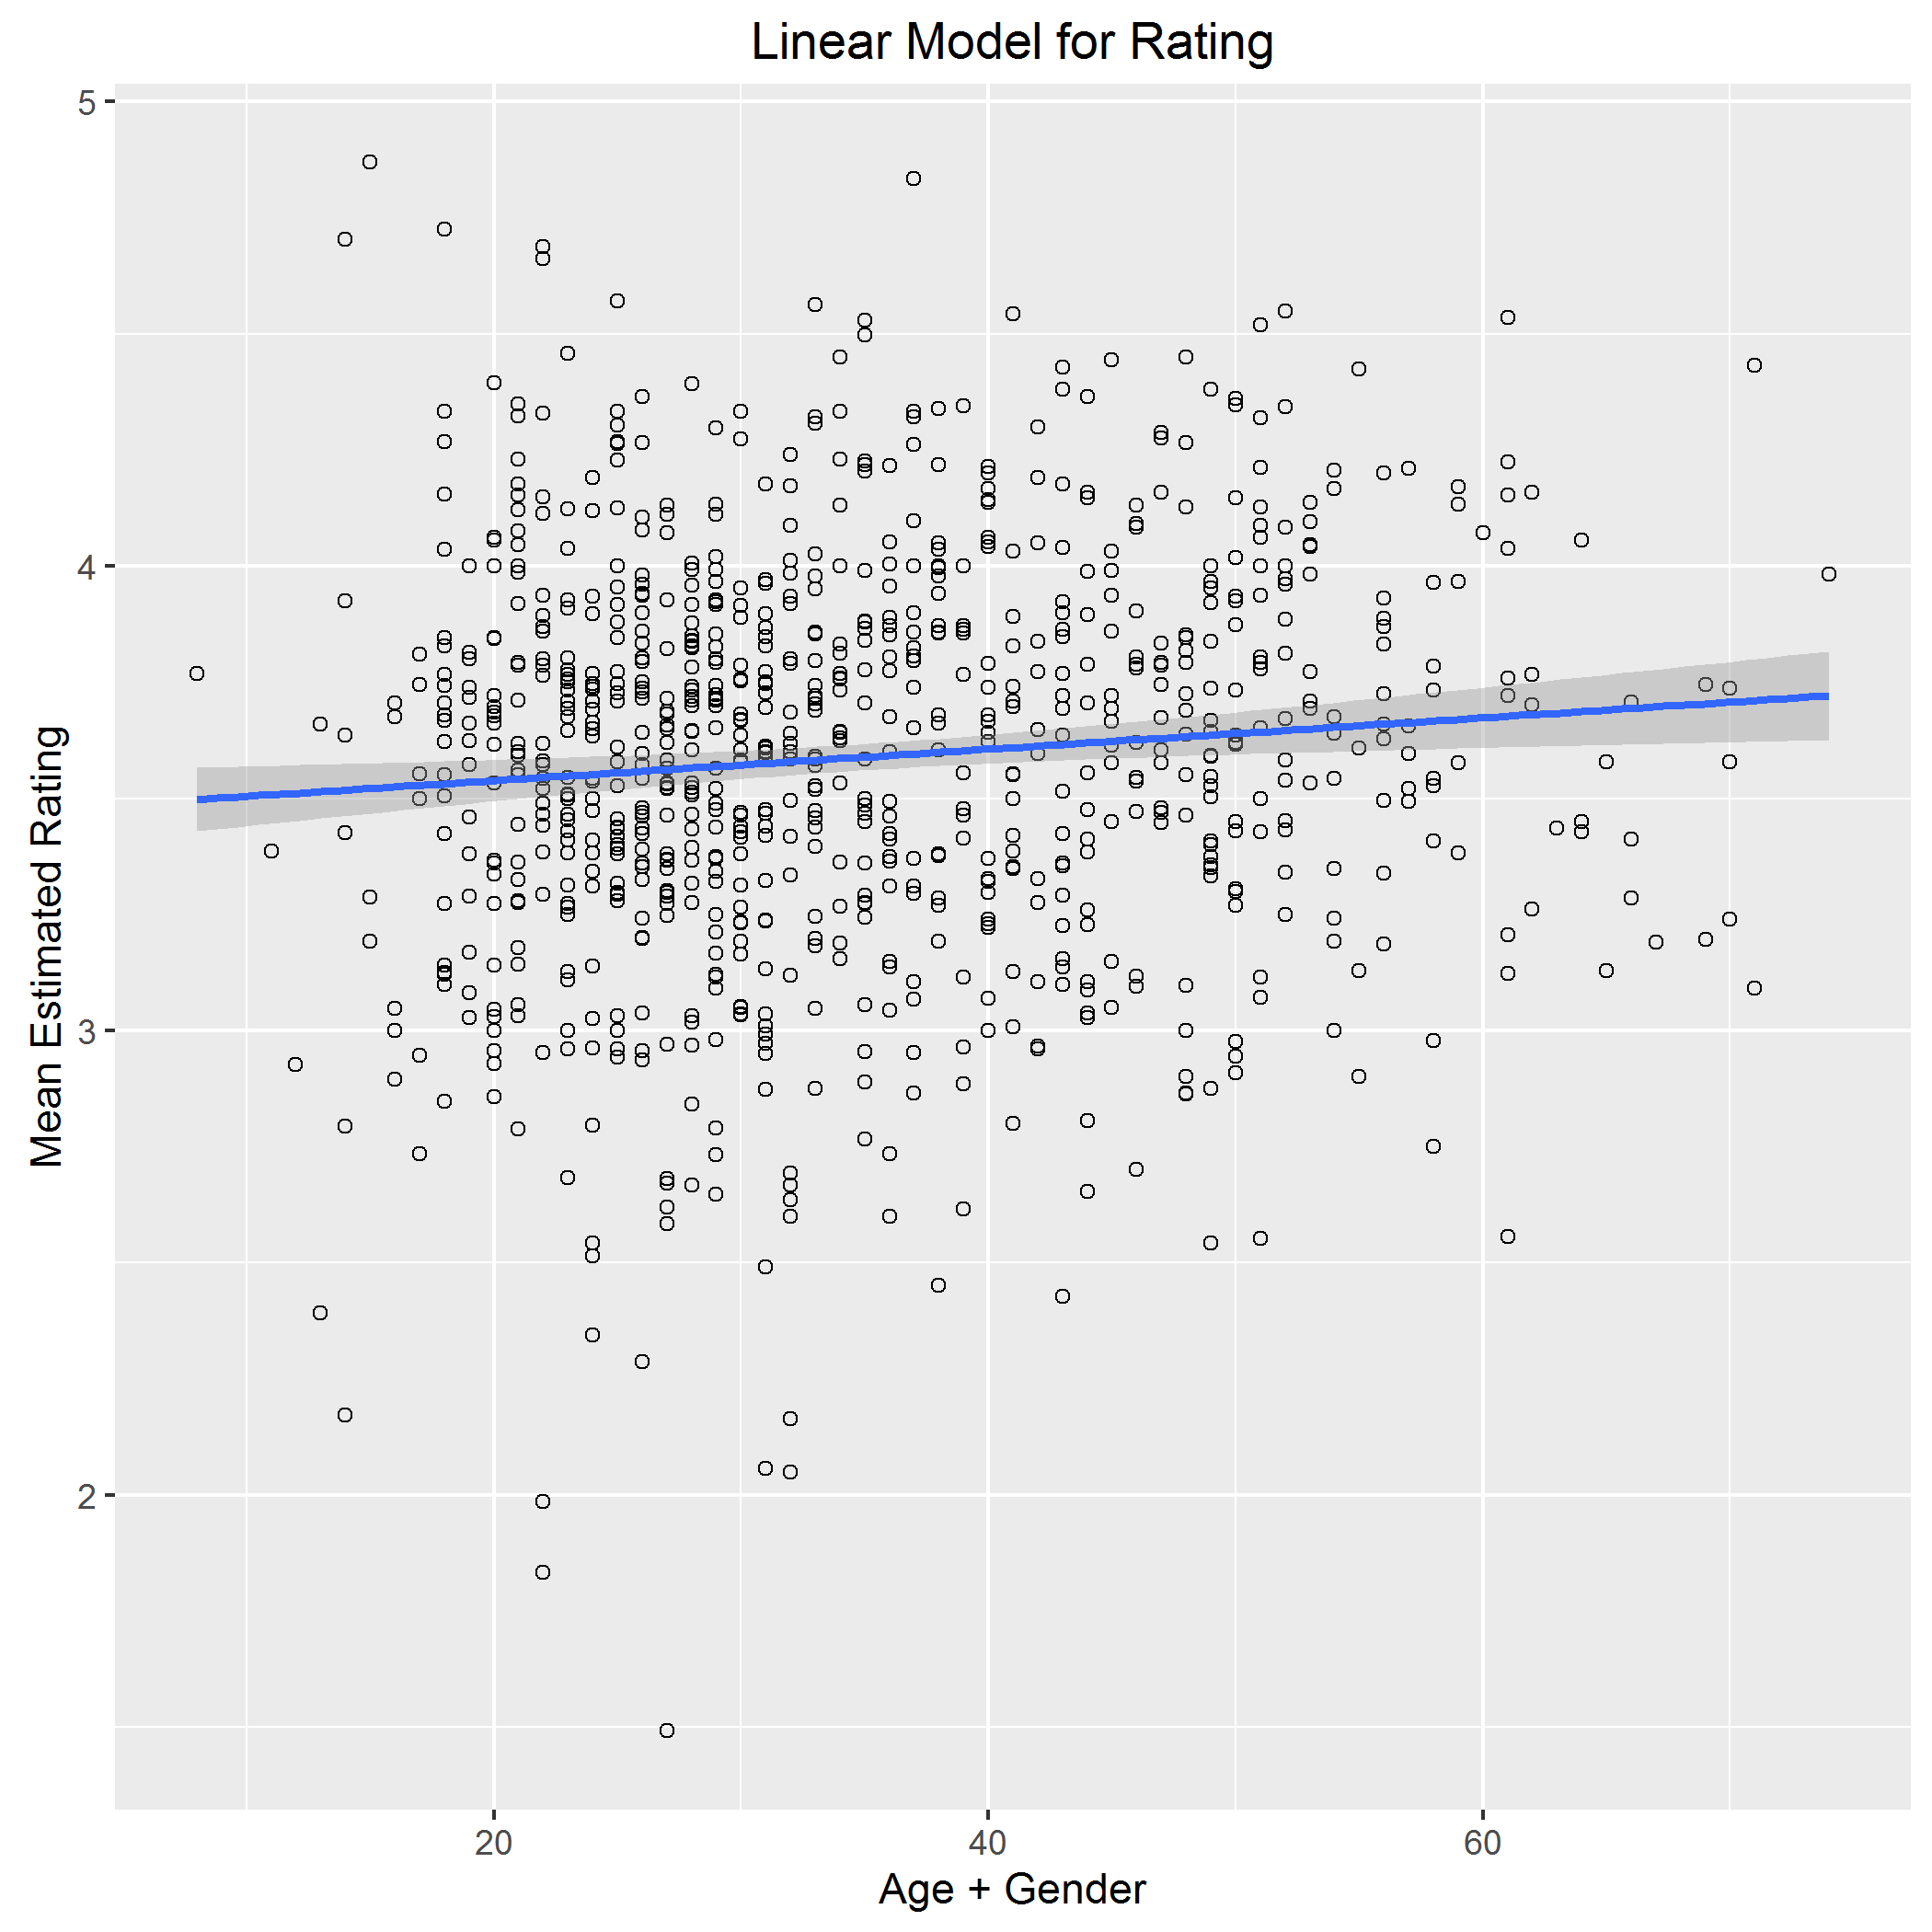
\includegraphics[scale=.50]{regression}
    \label{fig:regres}
    \end{figure}
    
    We can also find a confidencet interval for the coefficient $\beta_{age}$. From the output above, we know the estimate of $\beta_{age}$ is 0.0034, with a Standard Error of 0.0011. We can use these to find the interval:
    \begin{align*}
        (0.0011, 0.0058)
    \end{align*}
    From this, we can ascertain that the coefficient $\beta_{age}$ must fall somewhere between 0.0011 and 0.0058.
    
    Just as we did with d), we will test a hypothesis: $H_0 : \beta_{age} = 0$ The hypothesis that the above coefficient for $\beta_{age}$ is 0.\\
    For our hypothesis test, we can use the Standard Error we found in the summary above.
    Using the equation:
    \begin{align*}
        Z = \frac{\hat{\theta} - c}{s.e(\hat{\theta})}
    \end{align*}
    Where $\hat{\theta} = 0.0033891$, $c = \beta_{age} = 0$ and $s.e(\hat{\theta}) = 0.0011860$
    \begin{align*}
        Z = \frac{0.0033891 - 0}{0.0011860} = 2.857588
    \end{align*}
    This is larger than 1.98, and so we reject the hypothesis that $\beta_{age} = 0$.
    
    Next, with a similar call to lm() (see Appendix~\ref{sec:lmoutA} for the output of the lm() call), we can find a confidence interval for the mean population rating among women who are 28 years old:
    \begin{align*}
        (3.294, 3.846)
    \end{align*}
    This was found by fixing the $\beta$ values to $\beta_{gender} =$ Female and $\beta_{age} = 28$. From the output we found the estimated mean rating among woman who are 28 is 3.57 with a standard error of 0.1407.

    So now we are 95\% sure that the mean rating among woman who are 28 years old is in the interval above.

    \begin{figure}[p]
    \centering
    \caption{cap}
    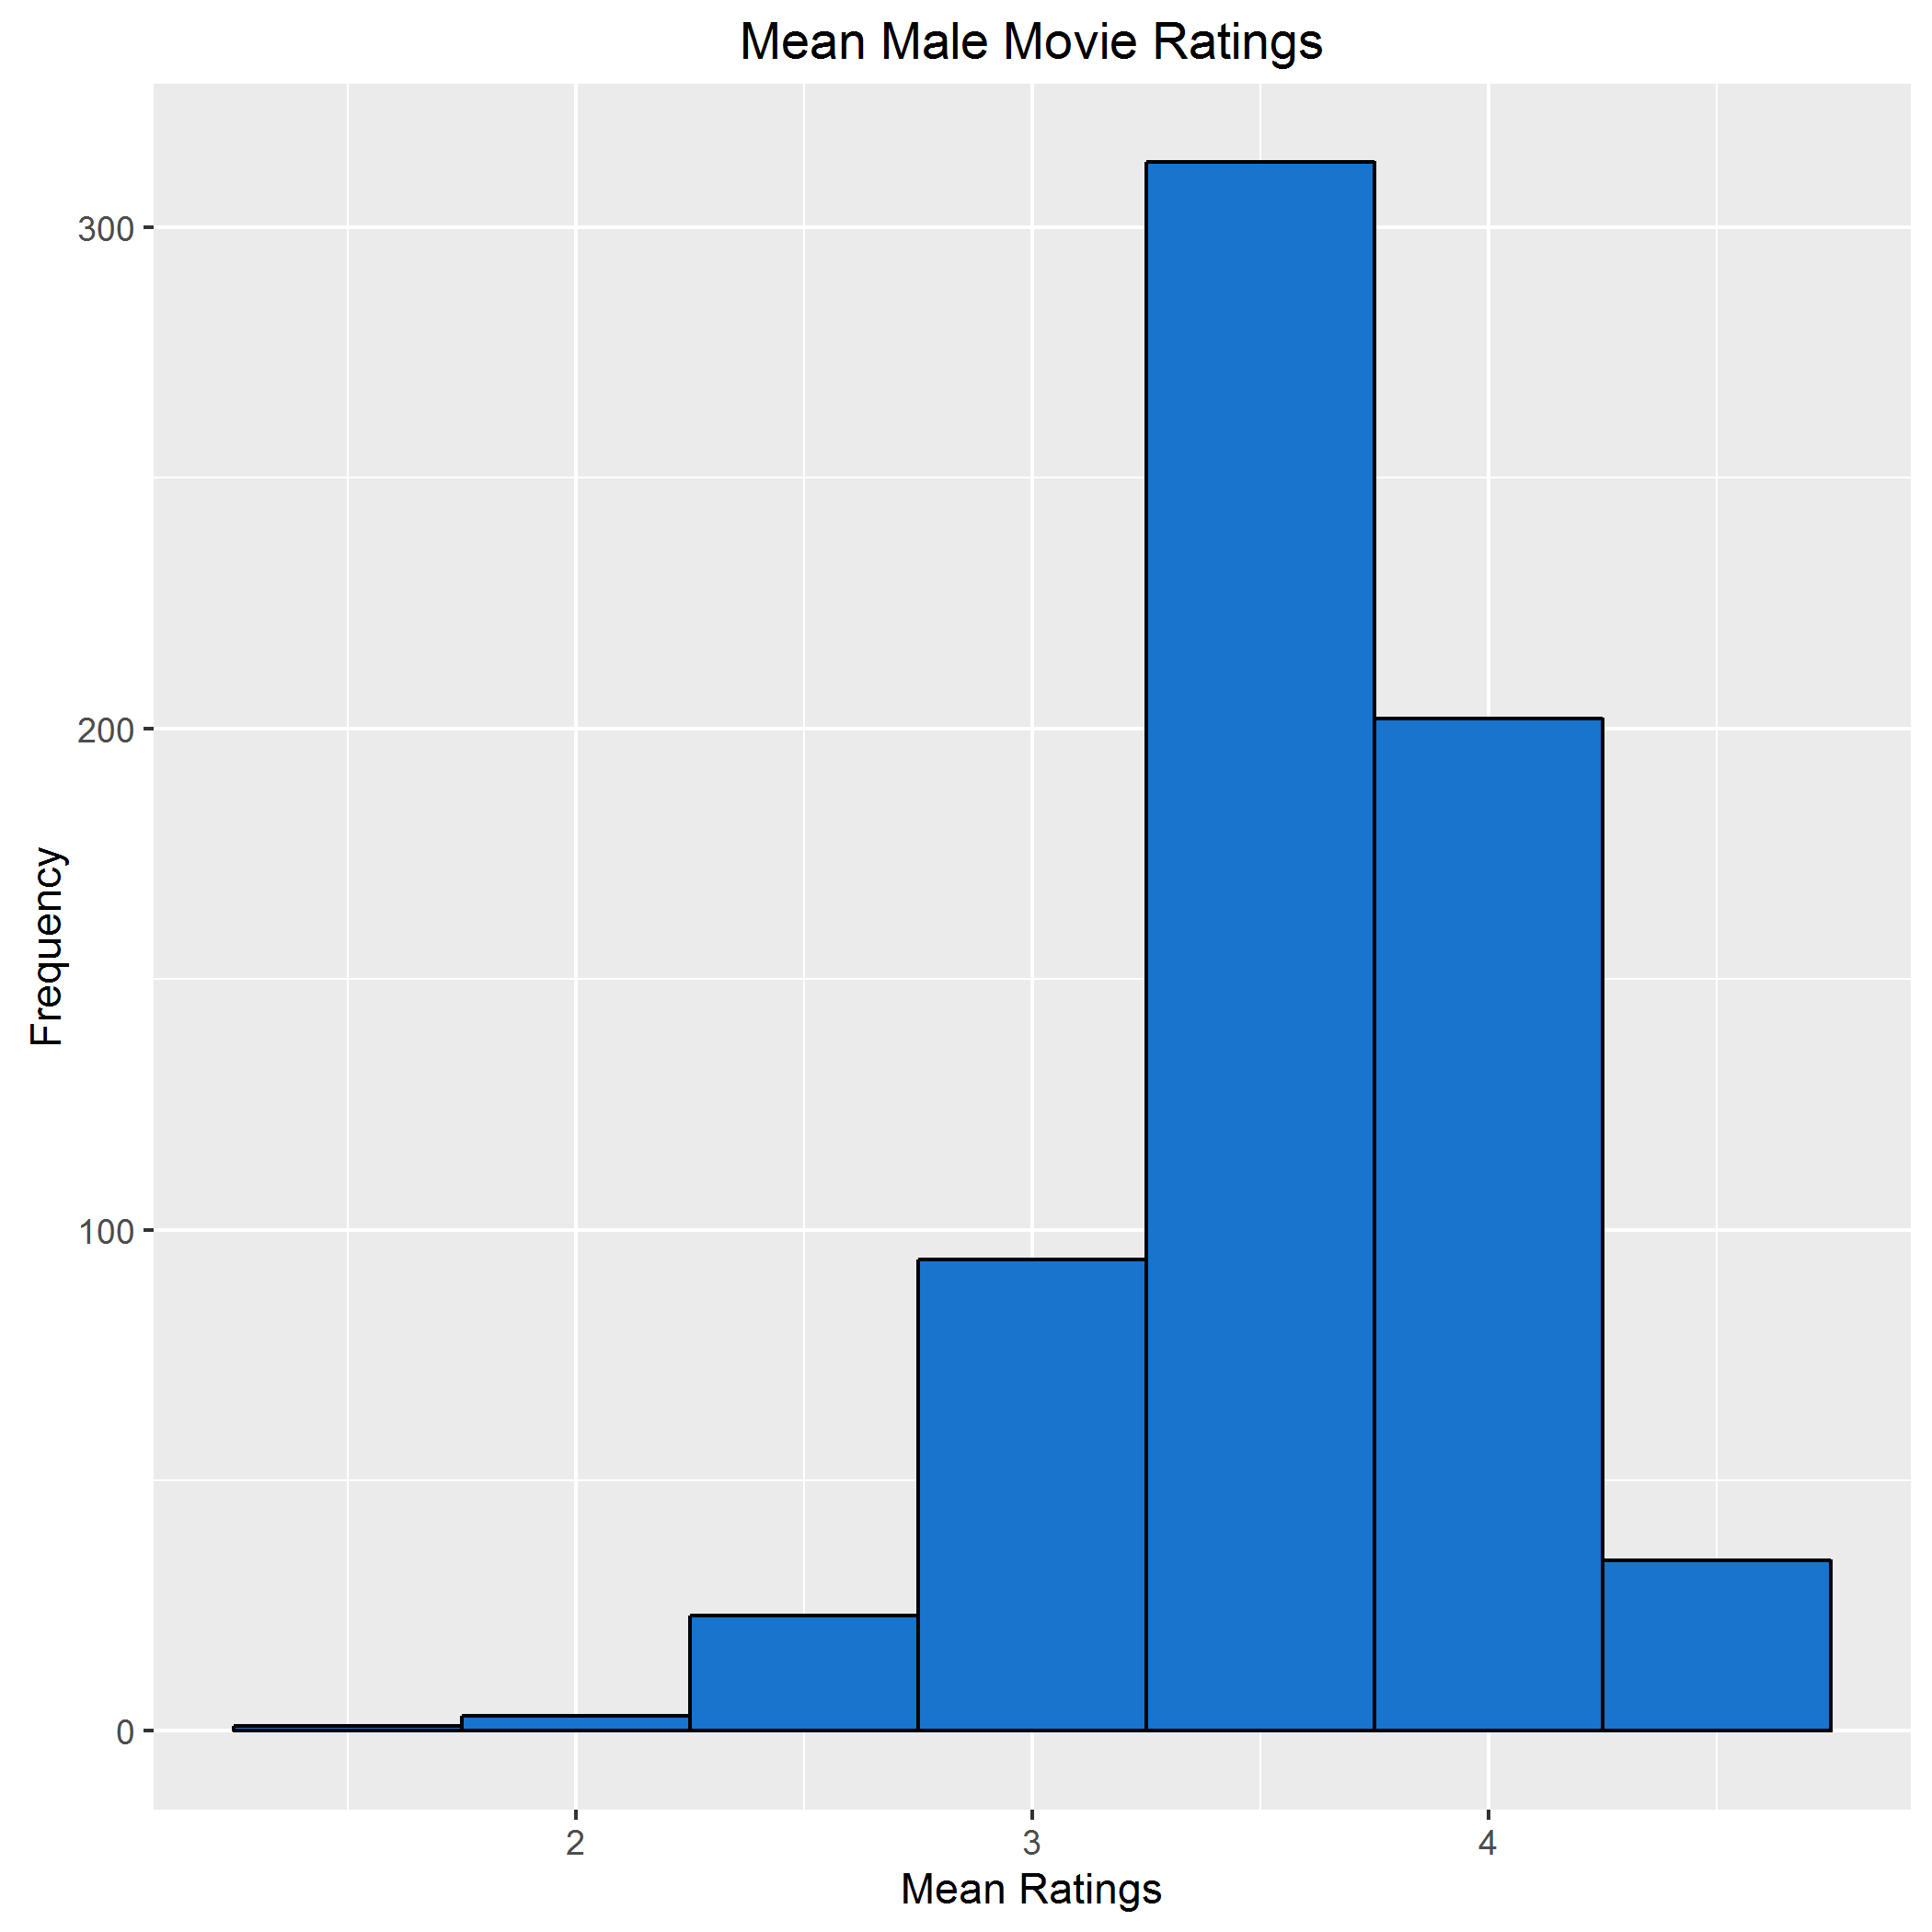
\includegraphics[scale=.50]{MaleHistogram}
    \label{fig:menhist}
    \end{figure}
    
    \begin{figure}[p]
    \centering
    \caption{TODO CAPTION}
    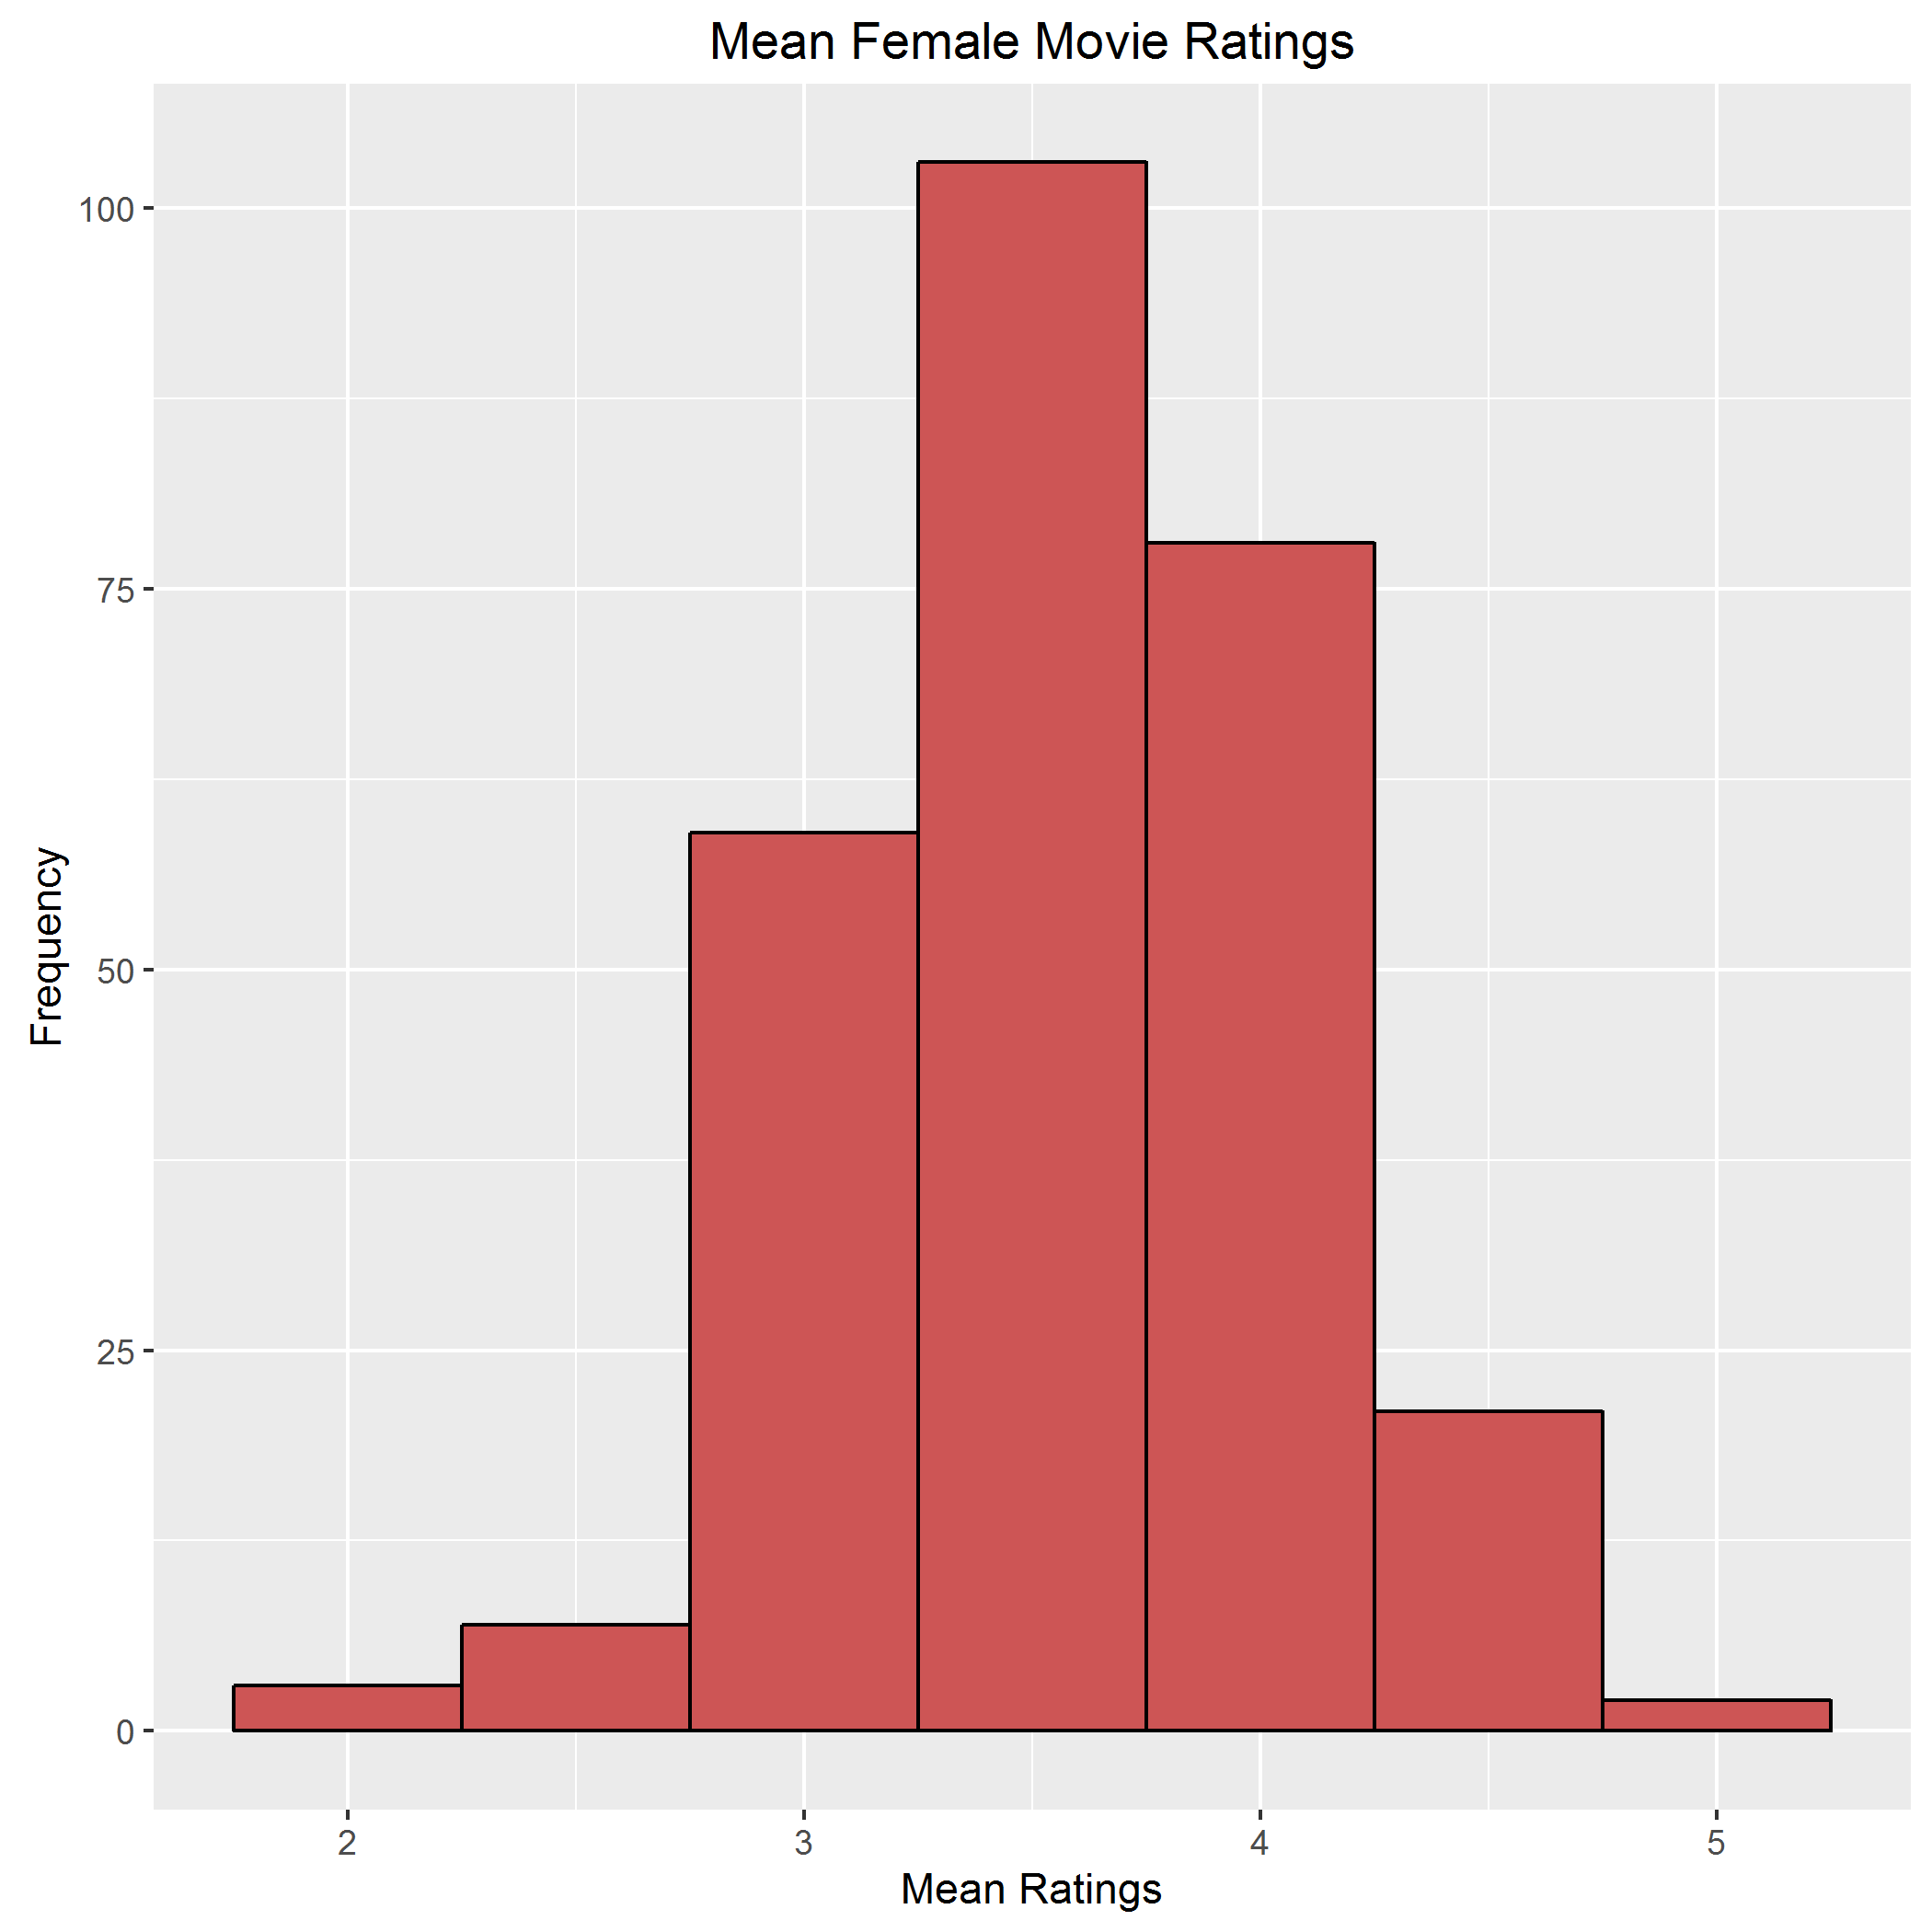
\includegraphics[scale=.50]{femaleHistogram}
    \label{fig:femalehist}
    \end{figure}
\end{enumerate}

\newpage
\addcontentsline{toc}{section}{Problem B}
\newpage
\begin{center}
\section*{Problem B}
\end{center}

\addcontentsline{toc}{subsection}{Introduction to .....}
%INTRODUCTION

\indent A study from Stanford utilizes questionnaires to collect data on a child's vocabulary development in various language, including factors such as their age, ethnicity, order of birth, gender, and mother's education. This data is open for public use as an online database called WordBank. One thing we could learn from this data is whether or not the mentioned factors have a strong effect on a child's English vocabulary size. We can explore this question by creating a regression model. By fitting the data into a linear function, factors included, we can see if there is a relationship among the variables included in the data.

\indent We will assume that our data is linear enough to implement linear regression function. Then, we identify which of the variables we deem independent and dependent. Since we are determining vocabulary size by the other variables, it will serve as our dependent variable for most of our analysis. The rest are independent variables which we will control to evaluate our dependent variable.

%Age and order of birth can be adjusted numerically, so we can use these as independent variables. The other variables, namely ethnicity, gender, and mother's education, are categorical variables. They contain a very discrete set of values that are qualitative, rather than quantitative like age.
%\indent We can also narrow down the predictability of our data using dummy variables. Let's return to our discussion about categorical variables. When we consider these qualitative variables in terms of code, we can create something we call dummy variables. These dummy variables, also called indicator variables, only hold the value of 0 and 1. We can use this to adjust our regression model to account for dichotomous situations, such as female or male.
%\indent In cases of categorical variables with more than two options, like ethnicity, we can divide the various options into several dummy variables. However, this presents a big problem. Say for example if we used a mother's education as a dummy variable, which for ease of discussion, we will call $X_0$. $X_0$ has about seven different options to choose from, so when we put this into our code, we'd end up with six to seven dummy variables. Then we start doing the same with the other categorical variables, which also have quite a lot of settings. From a programming standpoint, we would have to deal with a ridiculous amount of variables, which would overcomplicate the model. Using too many dummy variables may dilute the data. Thus, we must be careful about which dummy variables to consider, and we will choose them by observing obvious trends in our scatterplots and performing tests on our variables.
%should we briefly mention multicollinearity?
%also needs retooling for the final approach of this problem bc i wrote this while assuming that we were going to make one huge equation, which isn't the case.

\addcontentsline{toc}{subsection}{SubSection 1}
\textbf{Vocabulary and Age}

%SCATTERPLOT OF VOCAB SIZE VS. AGE
\begin{figure}[h]
\centering
\caption{Age Vocab TODO}
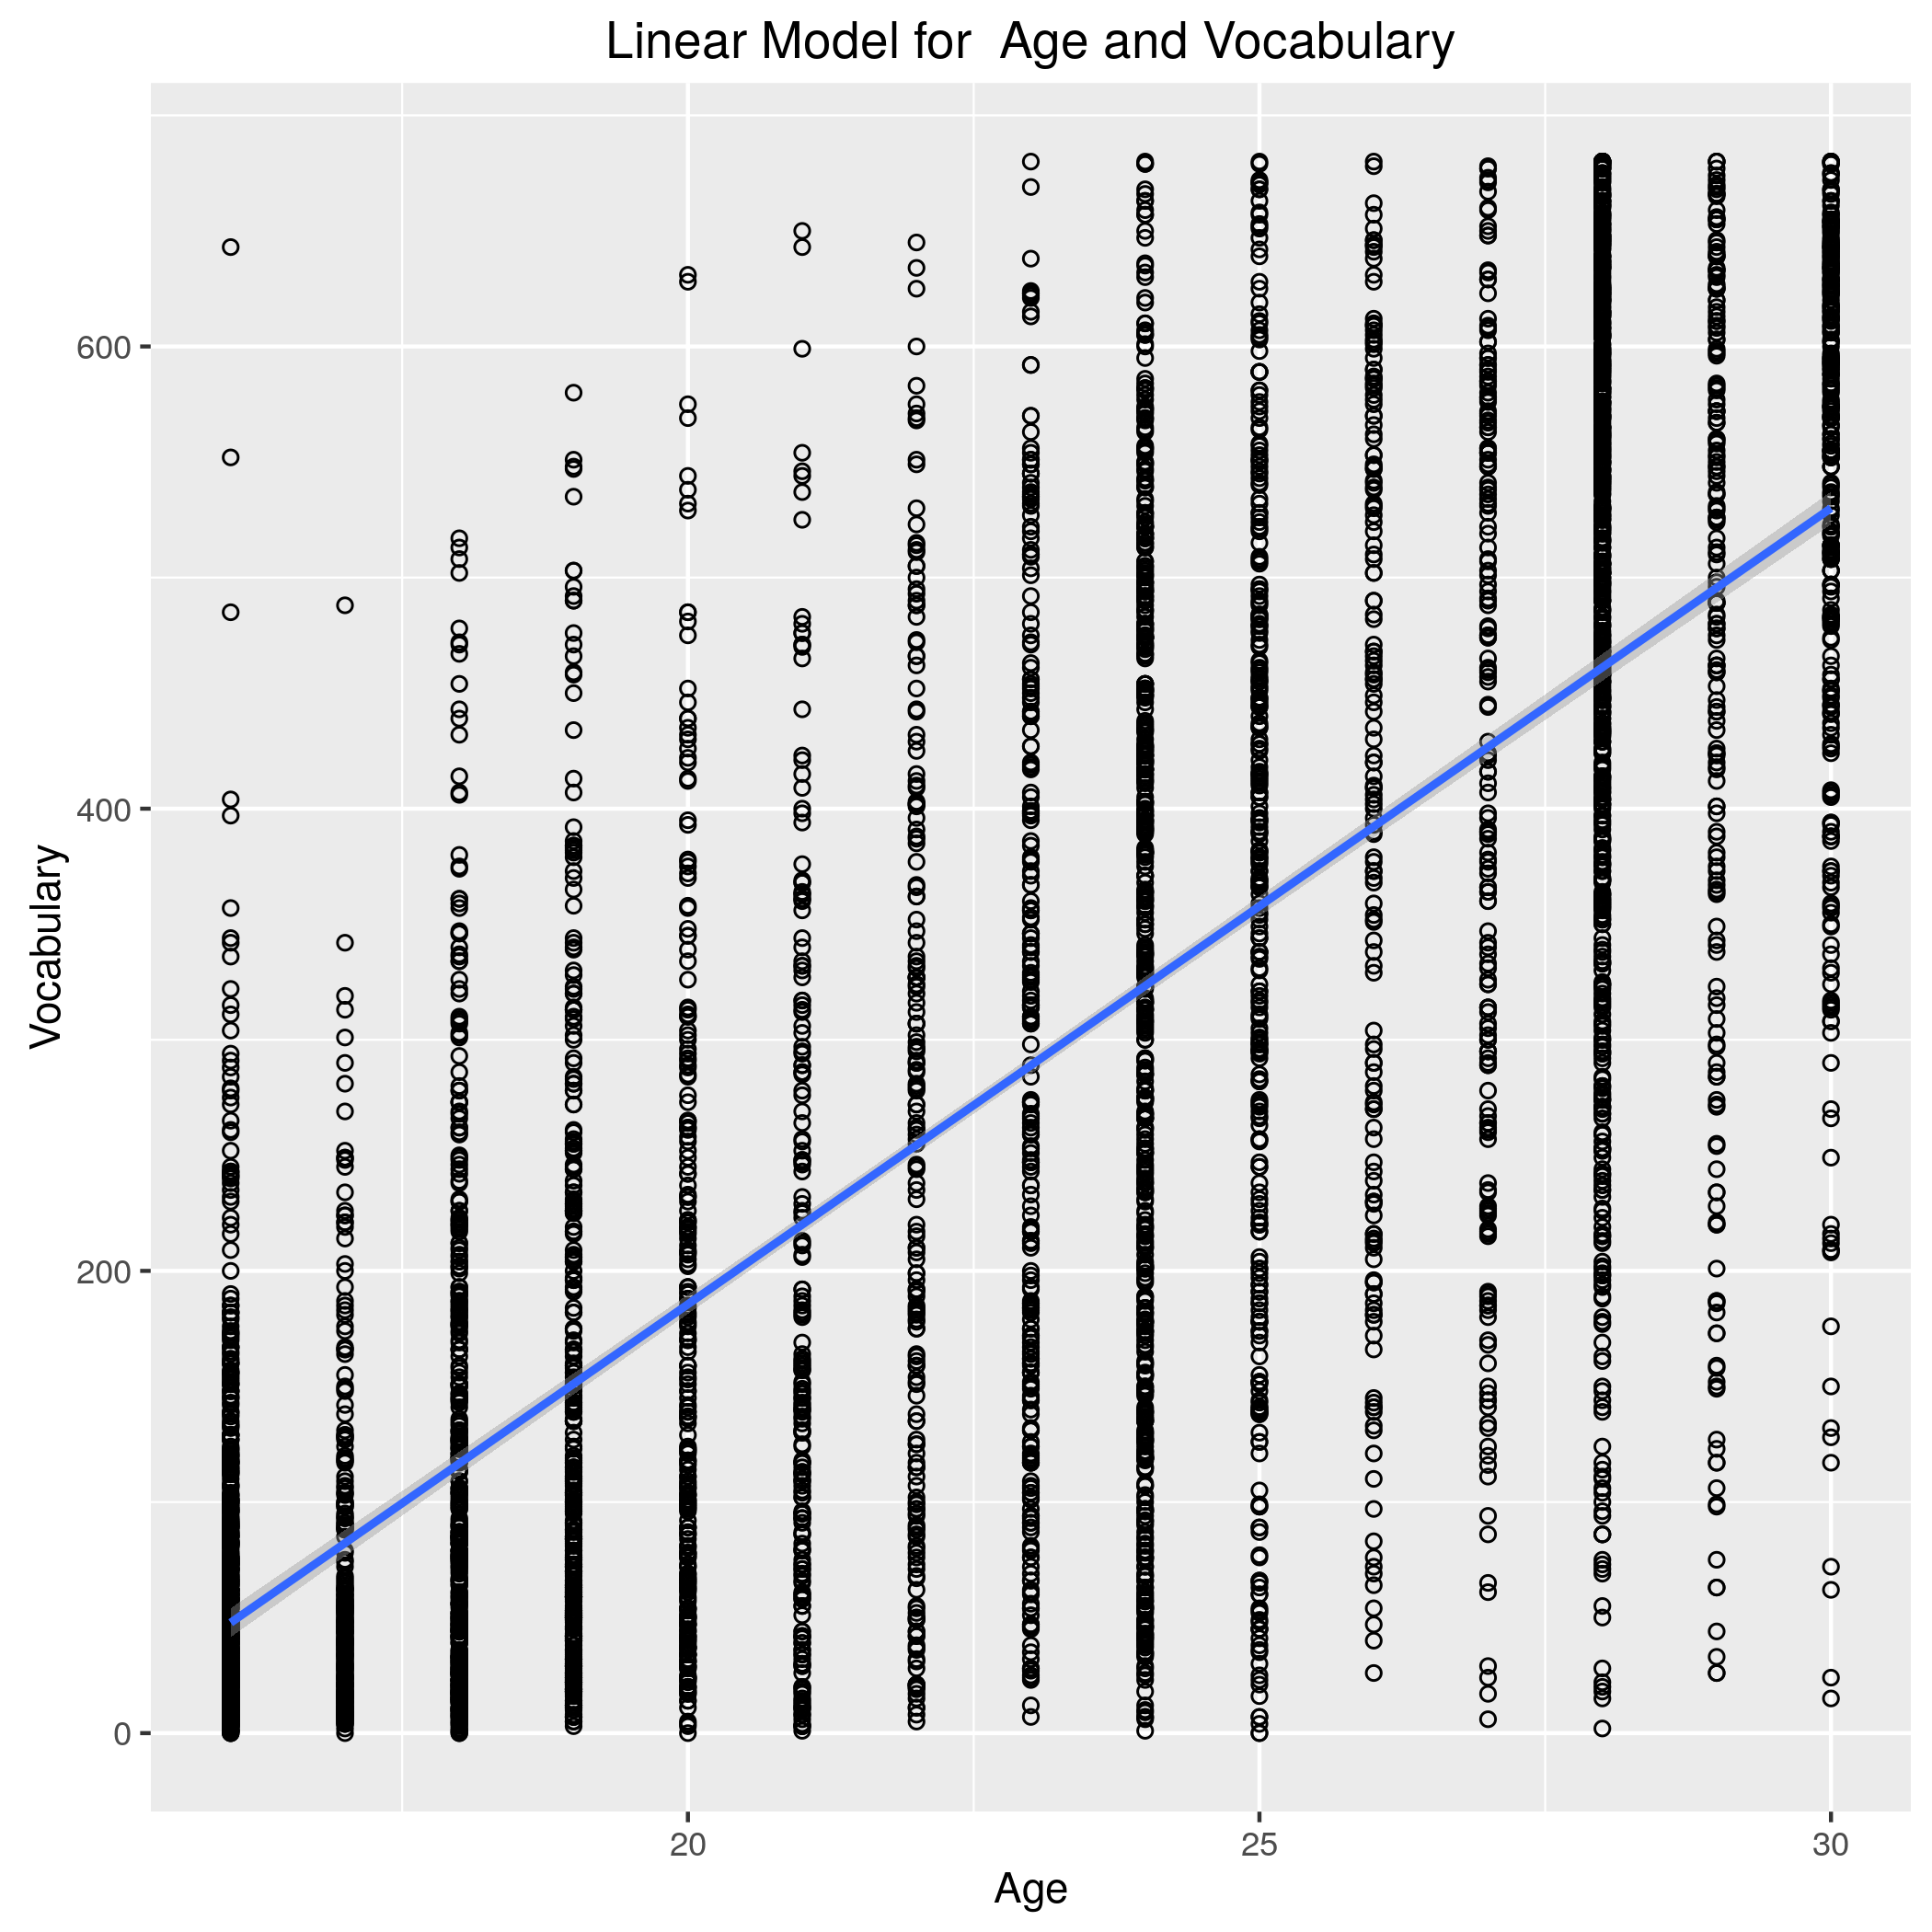
\includegraphics[scale=.50]{AgeVocab}
\label{fig:AVF}
\end{figure}

\indent We will first examine the relationship between vocabulary size and the child's age. We start out with the following regression function:
    \begin{align*}
        m_{S;A}(t) = \beta_0 + \beta_1 t_1
    \end{align*}
    In more colloquial terms:
    \begin{align*}
        \text{vocabulary size} &= \beta_0 + \beta_1\ \text{age}
    \end{align*}
\indent The $\beta$ can be considered constants that we will determine from our code later. What is important to note here is that we believe that for an increase in age, there will be an increase in vocabulary size.

\indent Now that we've determined the variables for our model, we can begin discussing the most important topic of verifying our regression function. Since we are using the regression function to create a best fit line that encompasses all our data, we naturally would want to know how well our data fits the function. We can use the built in R function lm() for linear models to perform a regression analysis as well as tests for correlation.

\indent We are given the confidence interval:
    \begin{align*}
        (3.294, 3.846)
    \end{align*}
    %VALUES NEED ADJUSTING
\indent %interpret confidence interval.


\indent We could do more tests on the various variables to see if we are good at predicting with this model, but we can easily see these details through more telling parts of the readout. The results of the call to lm() can be found in Appendix~\ref{sec:AVlm}. At the bottom of our results, we see the terms "R-squared" and "Adjusted R-squared". These numbers use a thing called residuals, which in simple terms are the distances each point of data is from the regression function. The quantity $R^2$ is an estimate of the correlation between vocabulary size and all the variables we used to predict it. The closer $R^2$ is to 1, a proportion of 100\% correlation, the better our data fits the model and the better our model can predict future cases.

\indent In the case of this regression function, $R^2$ only slightly above 0.5.
%it's a good model if the R^2 and R^2 adjusted is high. Our model is considered a good predictor if the R^2 predicted is also high.

\indent We plotted our data in Figure \ref{fig:AVF} and noted that there is a positive correlation between age and vocabulary size, as we had predicted earlier when we first formulated our regression function. Using the constants in our results, we have our complete regression function for age as a predictor of vocabulary size:
    \begin{align*}
        m_{S;A}(t) = 1.793 + 1.645 t_1
    \end{align*}

%conclusion to subsection: is this a good predictor?

\addcontentsline{toc}{subsection}{SubSection 2}
\textbf{Vocabulary and Ethnicity}

%SCATTERPLOT OF VOCAB SIZE VS. ETHNICITY
\begin{figure}[h]
\centering
\caption{Age Vocab TODO}
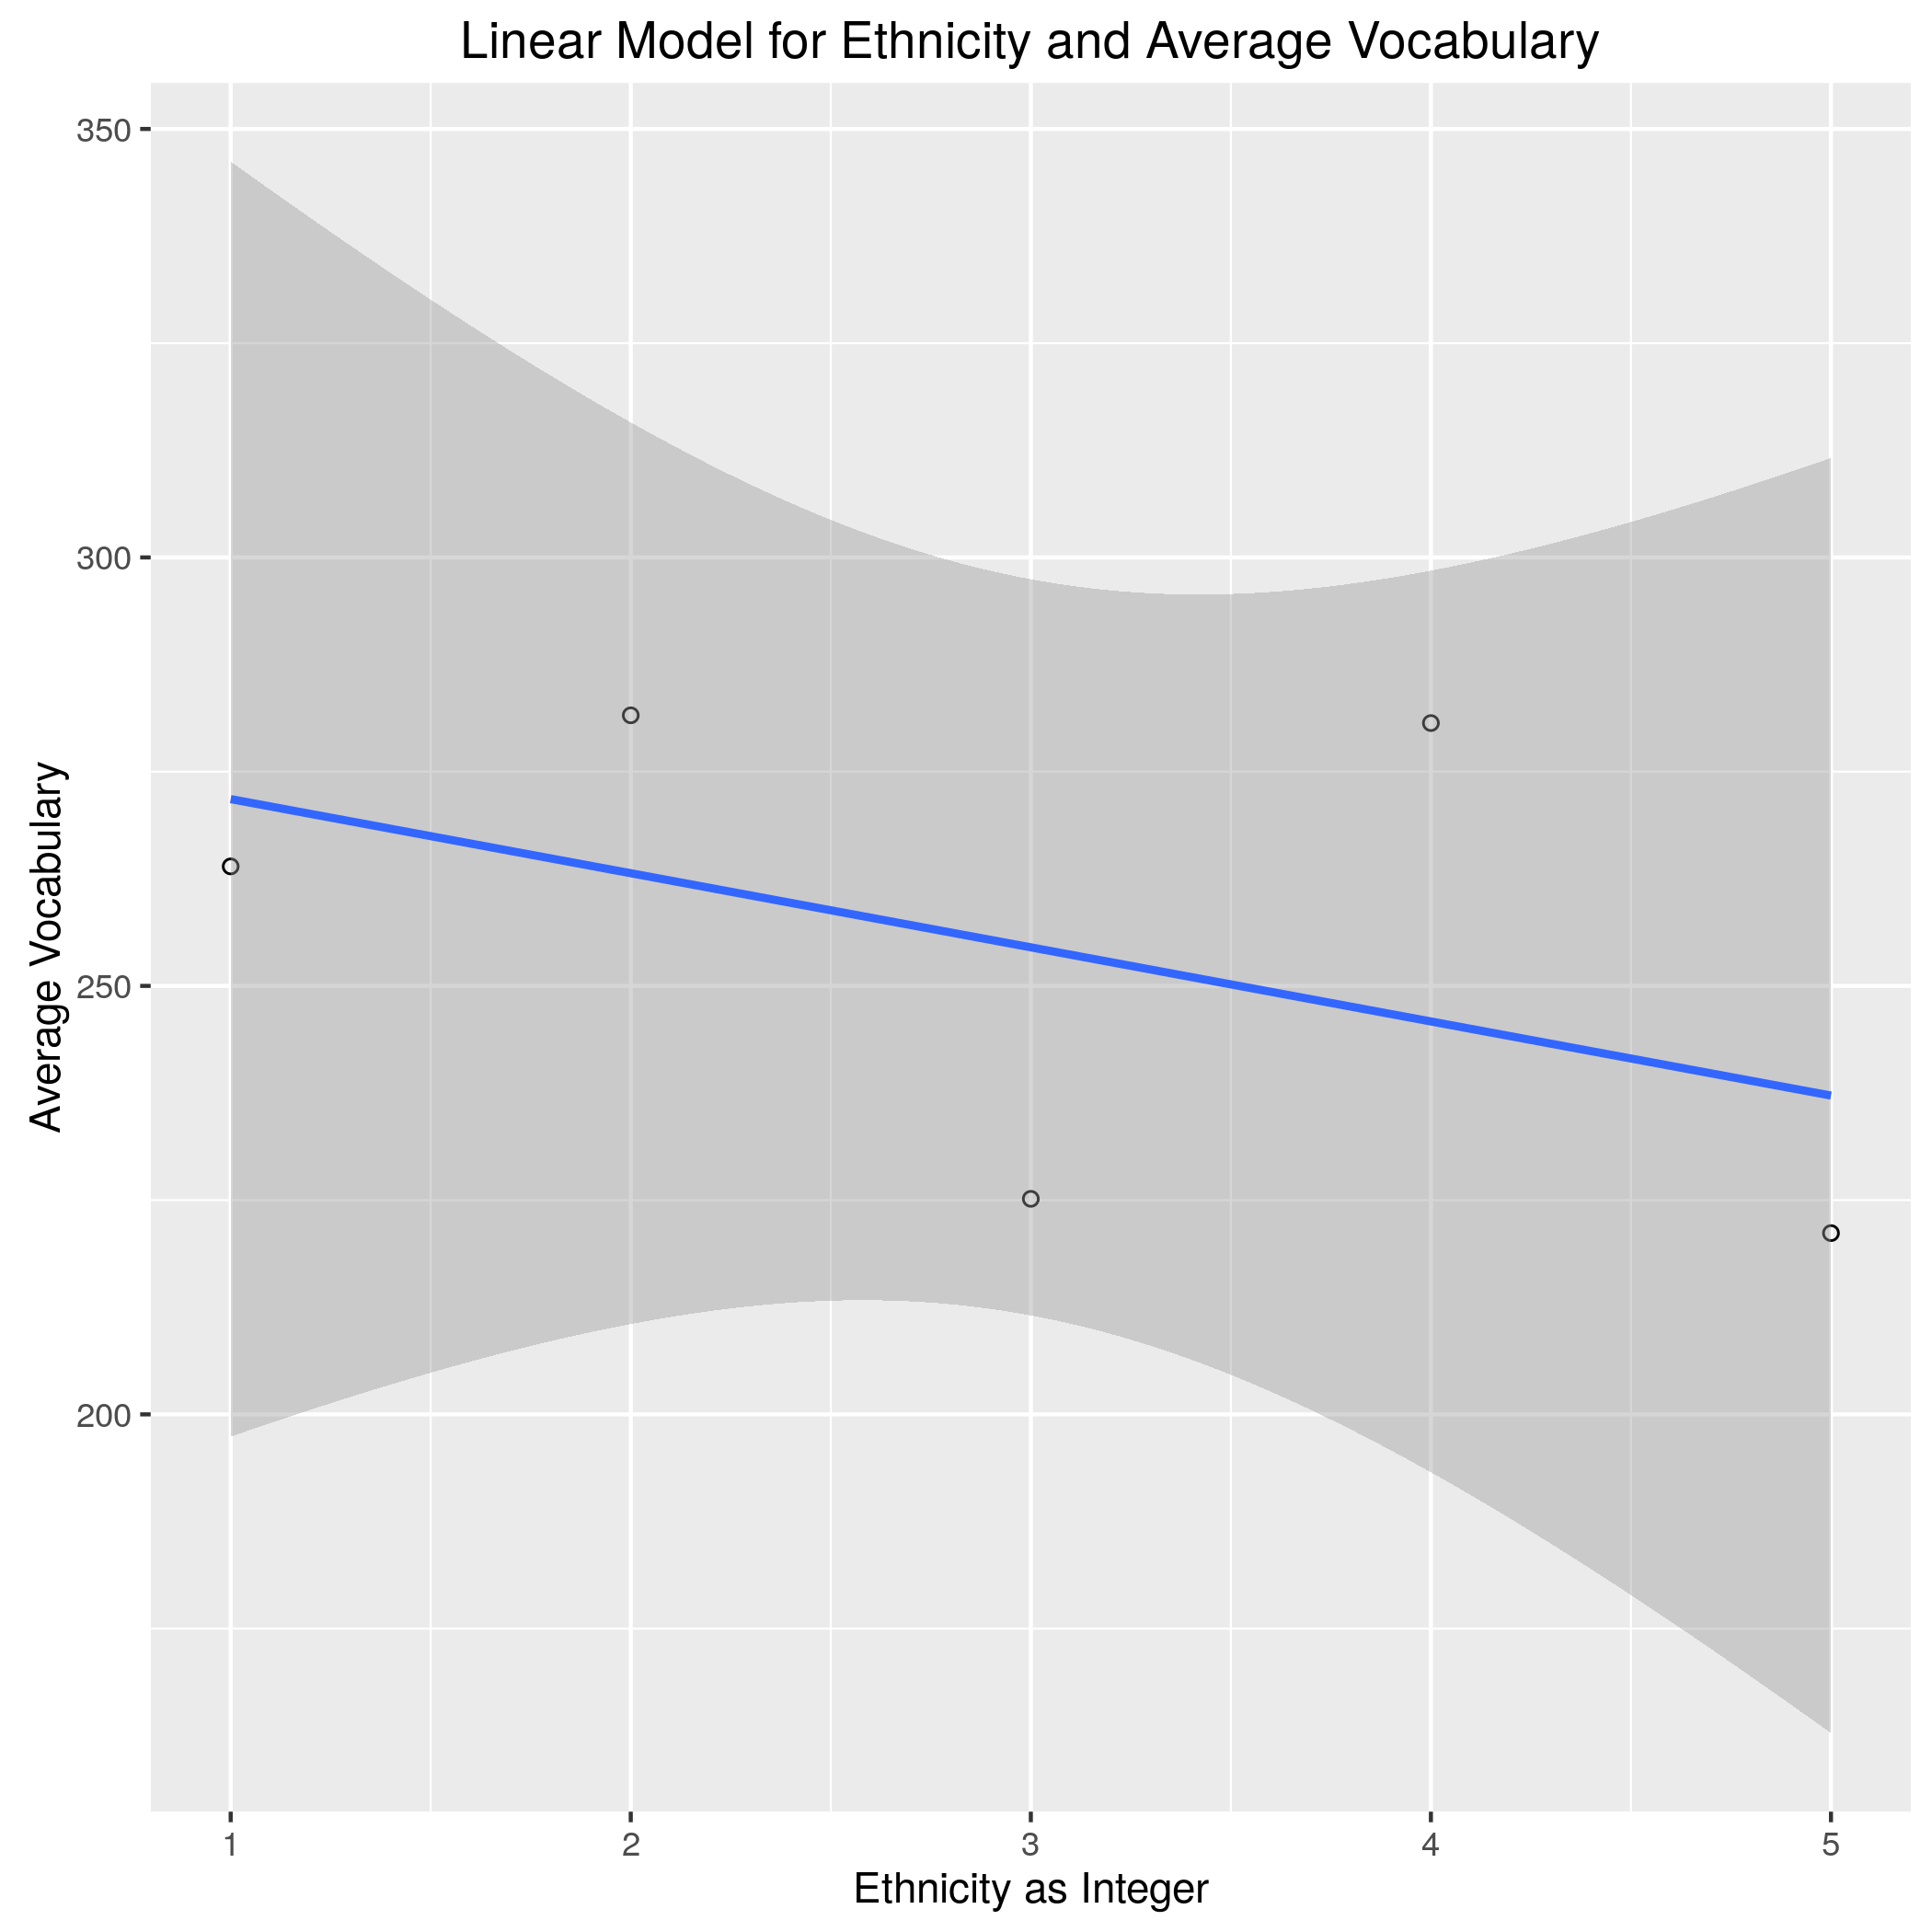
\includegraphics[scale=.50]{means_ethn}
\label{}
\end{figure}

\indent We repeat the same process as we had dont for age and vocabulary. But this time, we will look at how one's ethnicity can decide one's vocabulary size.

%explain why we put ethnicity in this manner.

%evaluate plot. positive or negative regression?
%tests, confidence intervals

%lm summary, look at R^2

%present final regression model with constants included

%conclusion to subsection: is this a good predictor?

\addcontentsline{toc}{subsection}{SubSection 3}
\textbf{Vocabulary and Sex}
%SCATTERPLOT OF VOCAB SIZE VS. SEX
\begin{figure}[h]
\centering
\caption{Age Vocab TODO}
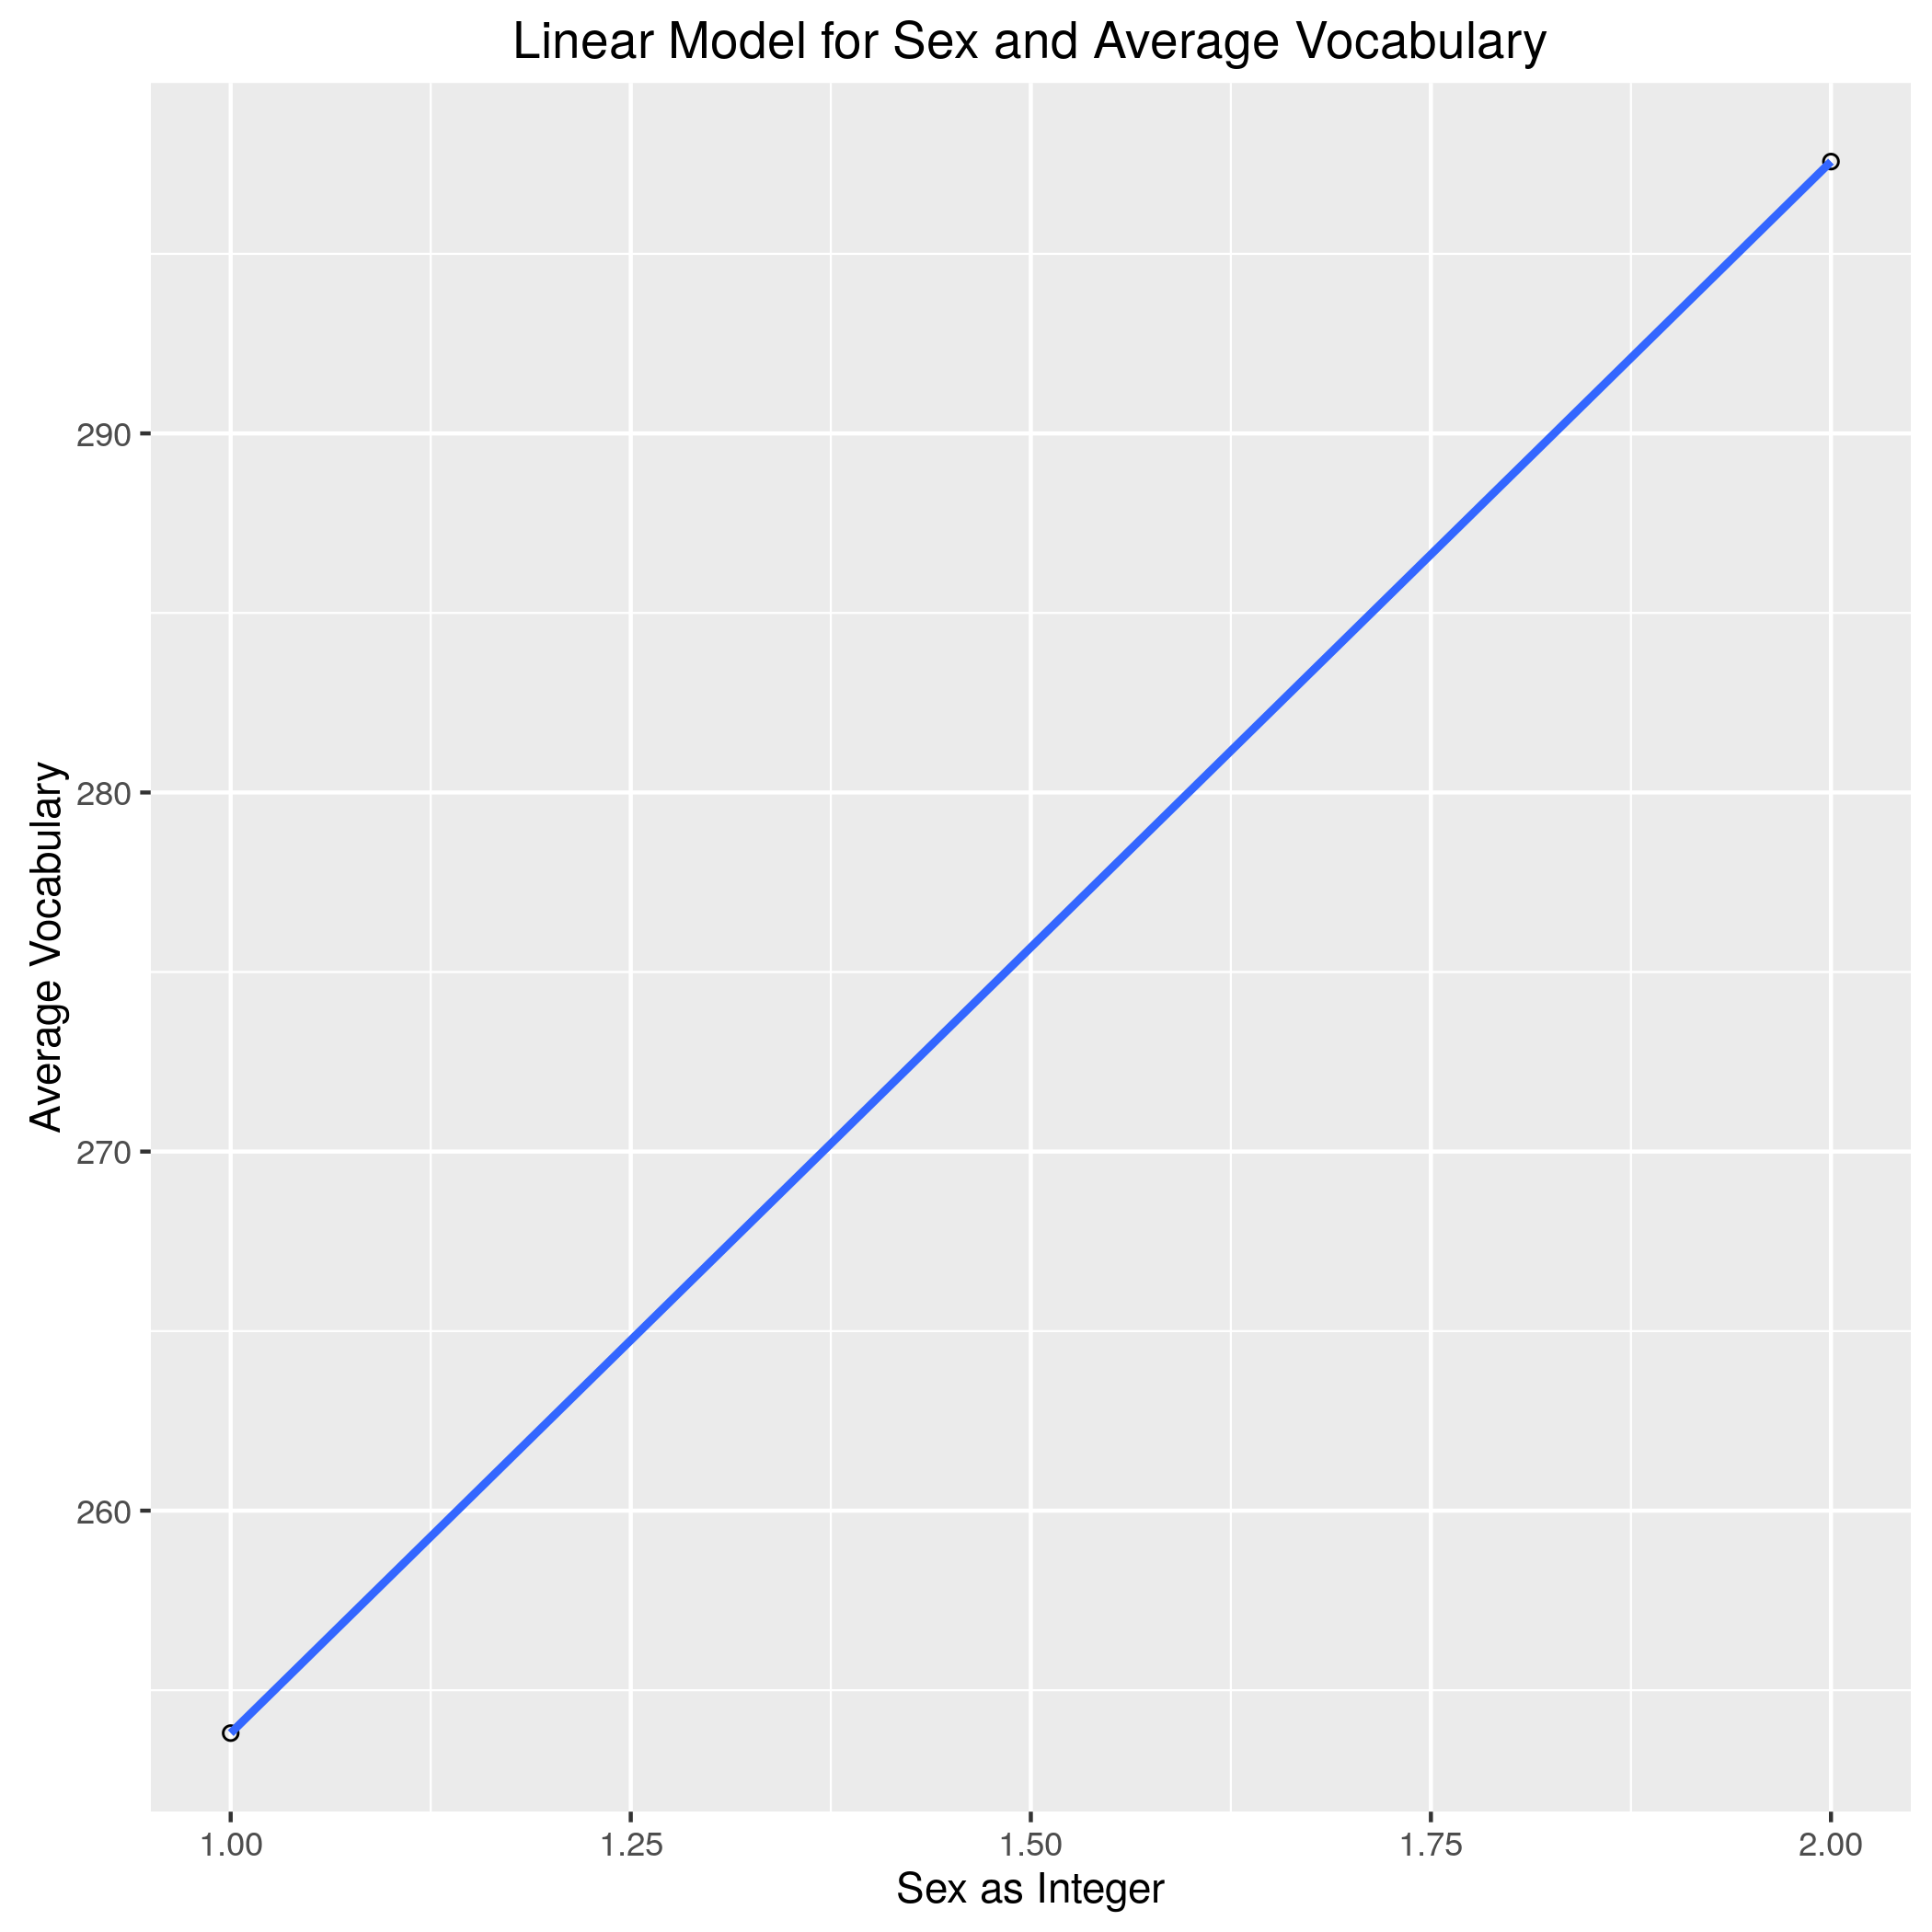
\includegraphics[scale=.50]{means_sex}
\label{}
\end{figure}

%explain why we put ethnicity in this manner.

%evaluate plot. positive or negative regression? In this case, we have something really weird here bc we only had two categories.
%tests, confidence intervals

%lm summary, look at R^2

%present final regression model with constants included

%conclusion to subsection: is this a good predictor?

\addcontentsline{toc}{subsection}{SubSection 4}
\textbf{Vocabulary and Mother's Education}
%SCATTERPLOT OF VOCAB SIZE VS. MOM'S EDUCATION
\begin{figure}[h]
\centering
\caption{Age Vocab TODO}
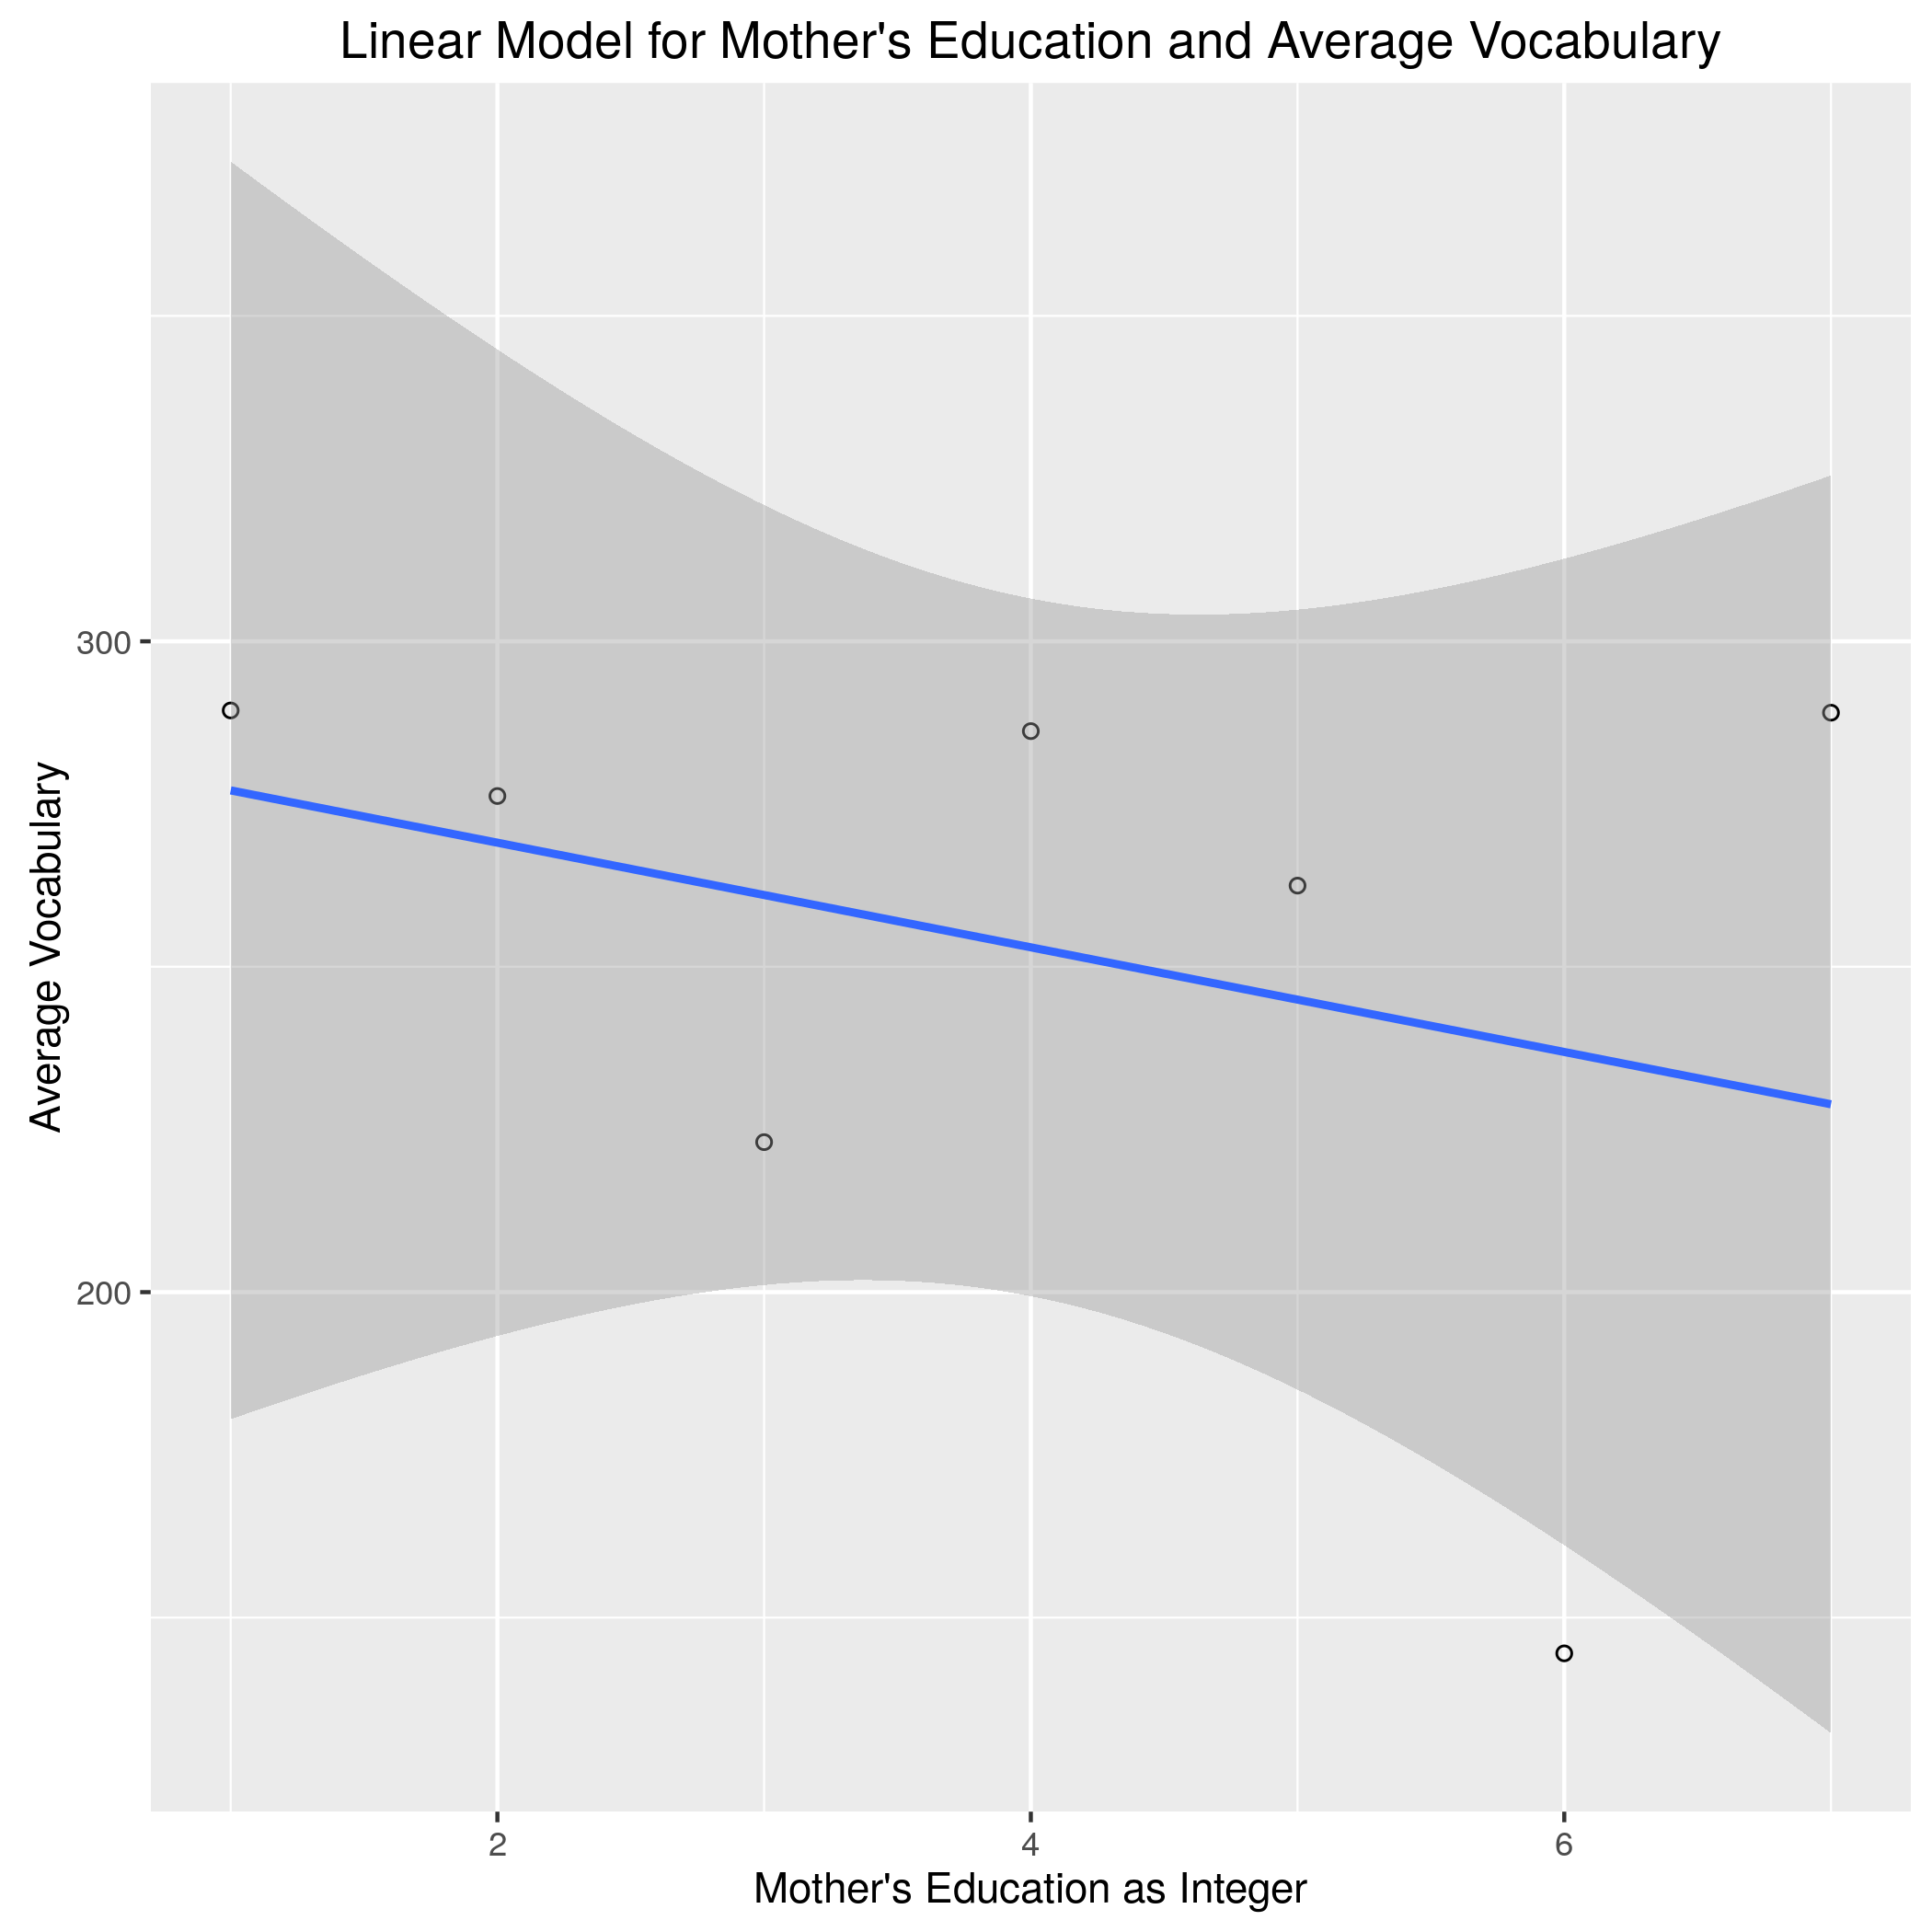
\includegraphics[scale=.50]{means_edu}
\label{}
\end{figure}

%explain why we put education in this manner. Although this variable is seemingly qualitative, we can treat it as quantitative because they are ranked.

%evaluate plot. positive or negative regression?
%tests, confidence intervals

%lm summary, look at R^2

%present final regression model with constants included

%conclusion to subsection: is this a good predictor?

\addcontentsline{toc}{subsection}{SubSection 5}
\textbf{Vocabulary and Order of Birth}
%subsection:BIRTH ORDER VS VOCAB SIZE
\begin{figure}[h]
\centering
\caption{Age Vocab TODO}
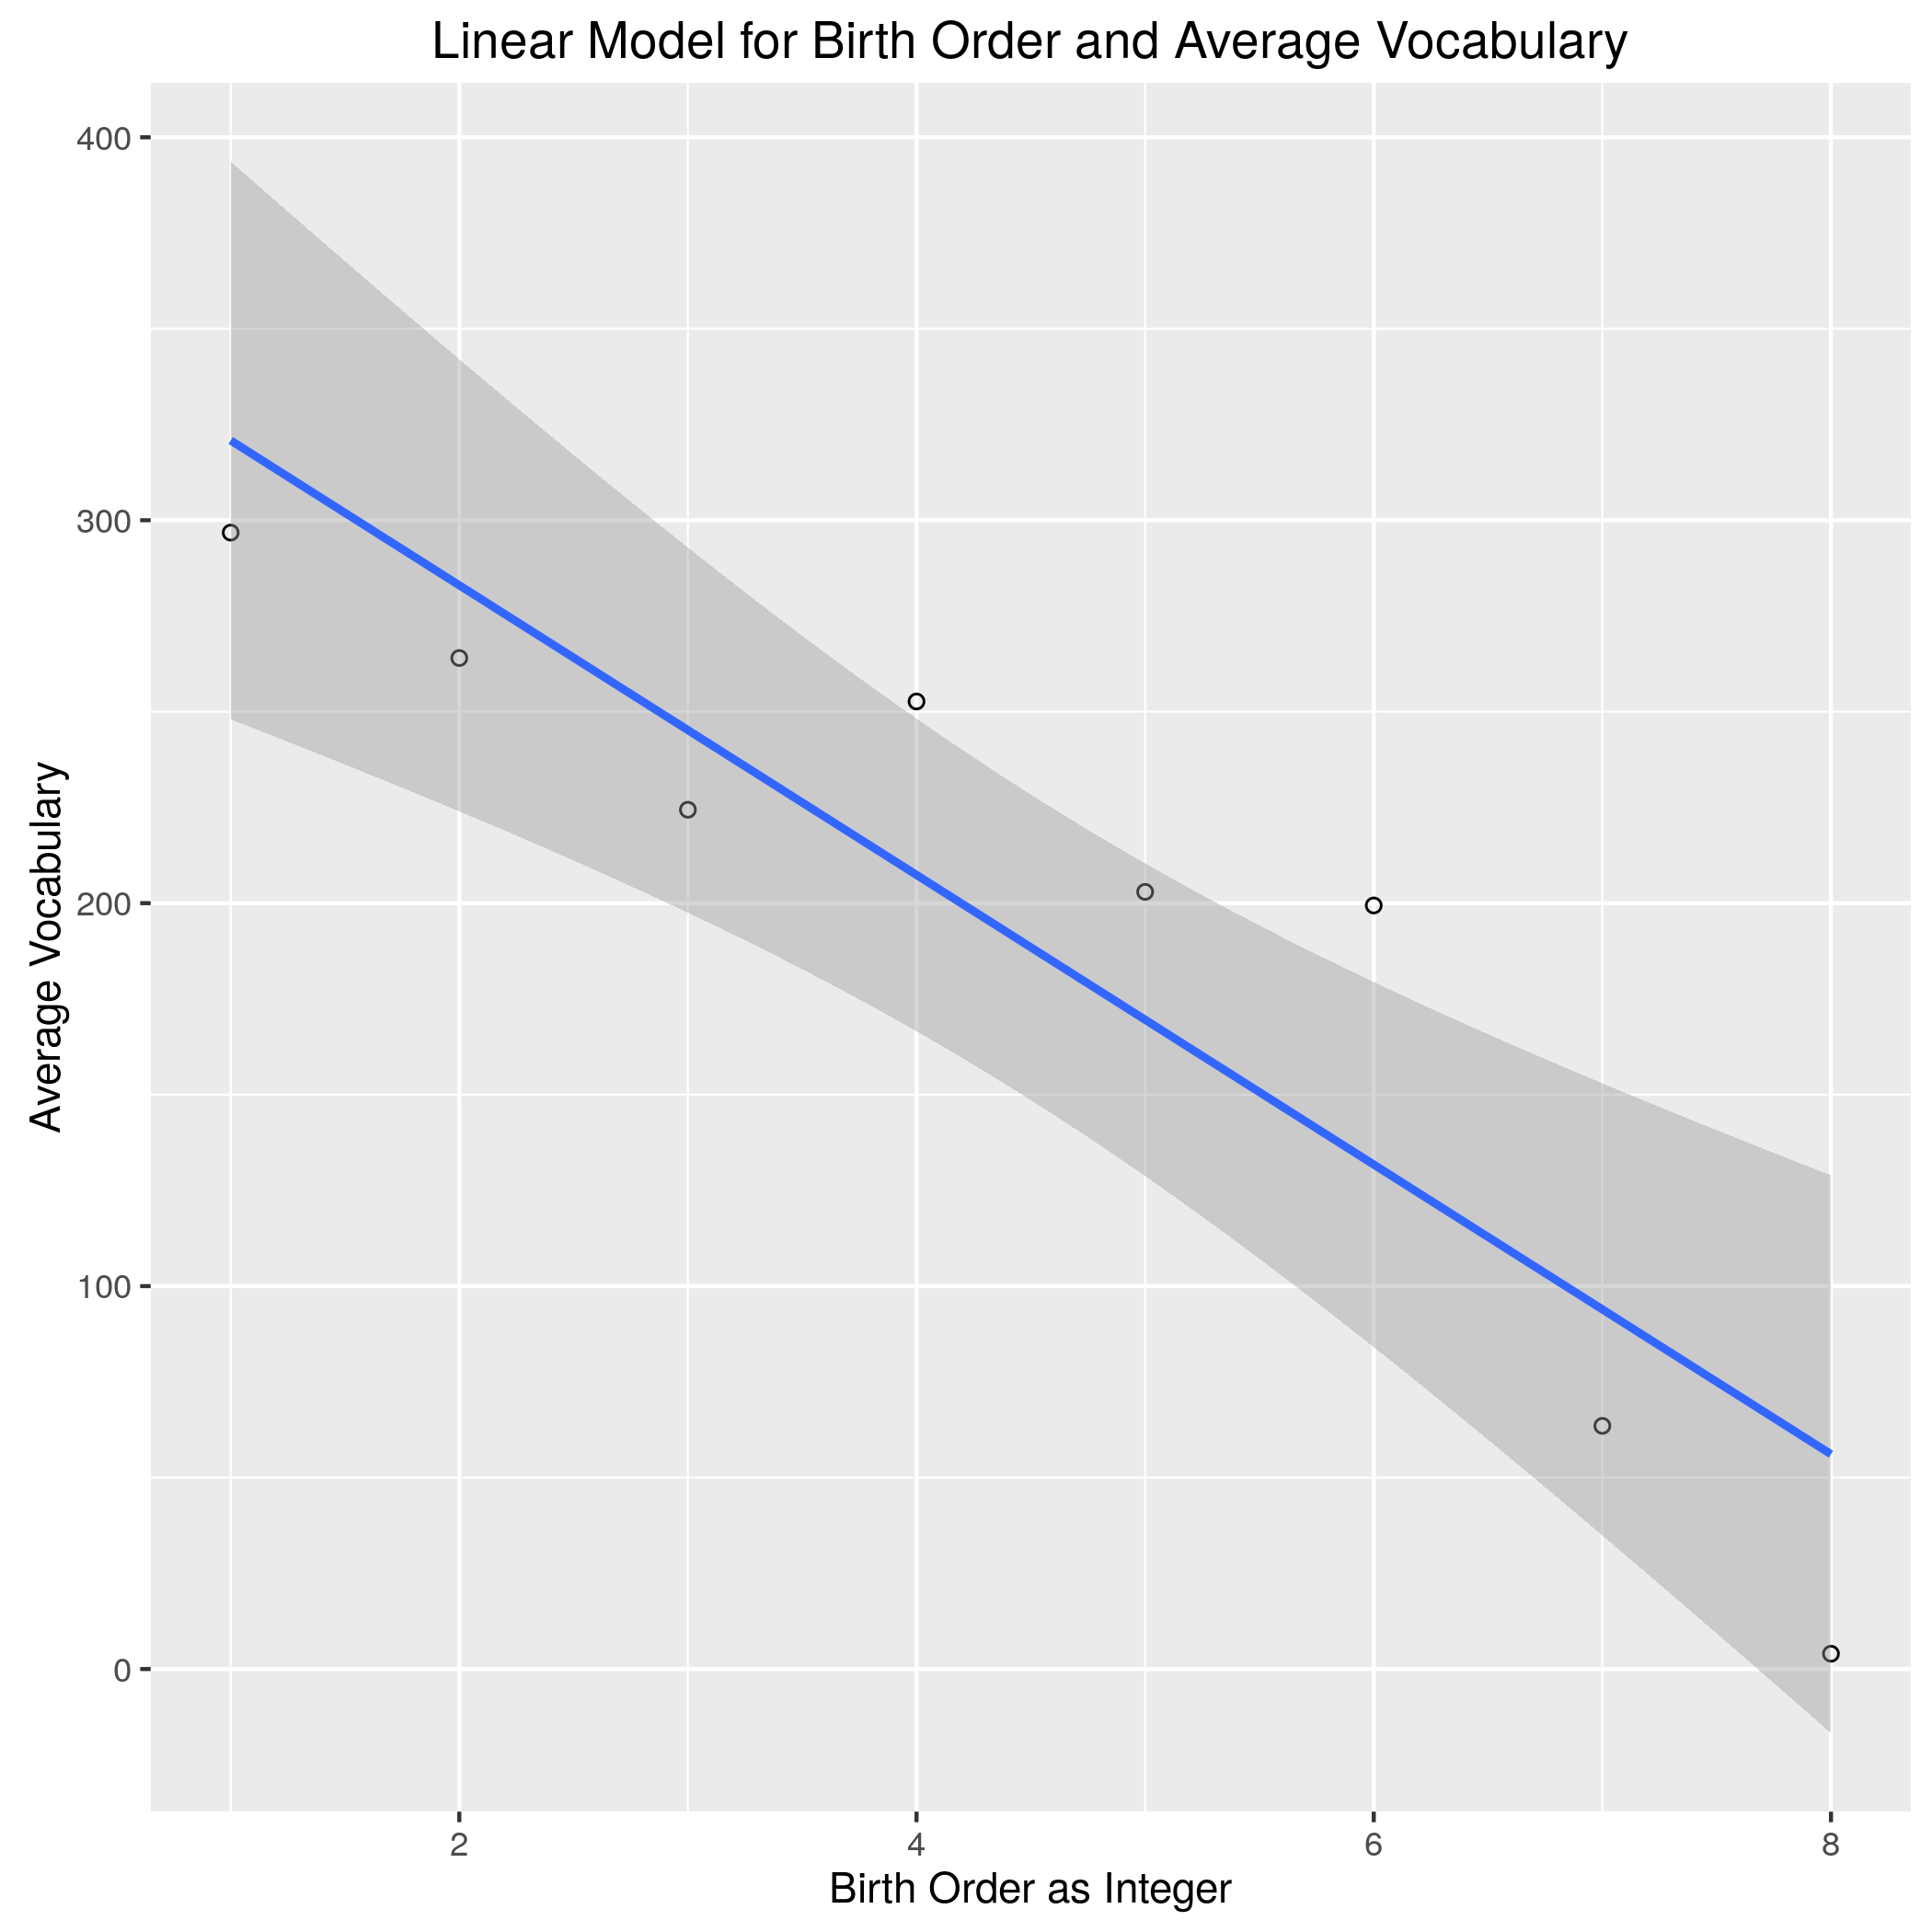
\includegraphics[scale=.50]{means_orders}
\label{}
\end{figure}
%SCATTERPLOT OF VOCAB SIZE VS. AGE WITH WITH COLORED POINTS DEPENDING ON BIRTH ORDER
%explain why we put birth order in this manner. Birth Order is quantitative, incidentally.

%evaluate plot. positive or negative regression?
%tests, confidence intervals
\indent We see from our plot that order of birth and their vocabulary size have a negative correlation.

%lm summary, look at R^2

%present final regression model with constants included

%conclusion to subsection: is this a good predictor?


%CONCLUSION
    %Which of the variables had the highest correlation?
    %What implications does this hold for predicting vocabulary size?
    %Any way to expand on our findings?

\newpage
\begin{center}
\appendix\section{Appendix}
\label{app}
\end{center}

%\addcontentsline{toc}{subsection}{Problem A General Functions}
\subsection{Problem A General Functions}
\label{sec:probagen}
Code that is indented is for readability and where code would wraparound.
\begin{itemize}
    \label{appendix:readData}
    \item The readData() function reads in the data from u.data.
    \begin{lstlisting}[basicstyle=\small]
    readData <- function()
    {
    	#Extracts the data from the file u.data with the following header
    	colNames <- c("UserID", "MovieID", "Rating", "Timestamp")
    	uData <- read.table("u.data", col.names = colNames)
    	
    	return(uData)
    }
    \end{lstlisting}
    
    \label{appendix:readUser}
    \item The readUser() function reads in u.user and returns the data in an appropriate data frame.
    \begin{lstlisting}[basicstyle=\small]
    readUser <- function()
    {
    	#Extracts the data from the file u.user with the following header
    	colNames <- c("UserID", "Age", "Gender", "Occupation", "ZipCode")
    	uUser <- read.table("u.user", sep = "|", col.names = colNames)

	return(uUser)
    }
    \end{lstlisting}
    

    \item mergeDataUser() merges the two data frames returned by readUser() and readData() into one single data frame
    \begin{lstlisting}[basicstyle=\small]
    mergeDataUser <- function()
    {
    	#Get the data frames for u.user and u.data
    	data <- readData()
    	user <- readUser()
    	n <- intersect(names(data),names(user))
    	#Merge them together where they intersect on headers
    	merged <- merge(data, user, by=intersect(names(data), names(user)))
    	#Write out to a file
    	write.table(merged, file = "u.merged", sep = "|", row.names = FALSE)
    	return(merged)
    }
    \end{lstlisting}
    

    \item getData() parses the information provided by mergeDataUser() into a useable data frame that is relevant to the problem. The data frame has the columns:\\
    UserID, Gender, MeanRatings
    \begin{lstlisting}[basicstyle=\small]
    getData <- function()
    {
    	#Get merged data to find the mean rating
    	userRatings <- mergeDataUser()
    	#Read in users to subset it for UserID and Gender
    	users <- readUser()
    	#Split the data from userRatings and find the mean of the ratings
    	# per user
    	ratings <- split(userRatings$Rating, userRatings$UserID)
    	Mean <- sapply(ratings, mean)
    	#Subset the user data frame to only UserID and Gender, and
    	# append on the Mean ratings per UserID
    	A <- subset(users, select=c("UserID", "Gender"))
    	A$Mean <- c(Mean)
    
    	return(A)
    }
    \end{lstlisting}
    
    \item getDataNum() is similar to getData(), but instead of appending the Mean ratings per user ID, it returns a data frame with the full non-aggregated user ratings
    \begin{lstlisting}[basicstyle=\small]
    getDataNum <- function()
    {
    	#Get merged data for all ratings
    	userRatings <- mergeDataUser()
    	#Get user data
    	users <- readUser()
    	#Subset the data by UserID, Gender, and Ratings
    	A <- subset(userRatings, select=c("UserID", "Gender", "Rating"))
    
    	return(A)
    }
    \end{lstlisting}
\end{itemize}

%\addcontentsline{toc}{subsection}{Problem A Confidence Interval Functionss}
\subsection{Problem A Confidence Interval Functions}
\label{sec:probaconf}
\begin{itemize}

    \label{sec:CIM}
    \item confIntMen() finds the approximate 95\% confidence interval for the population mean rating by men. Utilizes the function getData() in~\ref{sec:probagen} and equation (10.14) from "From Algorithms to Z-Scores"
    \begin{lstlisting}[basicstyle=\small]
    confIntMen <- function()
    {
    	#Get the data for Mean User Ratings
    	A <- getData()
    	#Get a subset of only males
    	men <- A[A$Gender=='M',]
    	
    	#Xbar - sample mean
    	sampleMean <- mean(men$Mean)
    	#n - sample population
    	samplePop <- nrow(men)
    	#sigma - standard deviation
    	stdd <- sd(men$Mean)
    	#1.96*s.e(theta) = the standard error applied to 95%
    	# interval
    	#Uses the equation sigma / sqrt(n)
    	error <- qnorm(0.975)*stdd/sqrt(samplePop)
    	#Find the left and right ends of the interval
    	# Xbar -+ error
    	left <- sampleMean - error
    	right <- sampleMean + error
    
    	cat("Sample Mean: ", sampleMean, "\n")
    	cat("Sample Population: ", samplePop, "\n")
    	cat("St Dev: ", stdd, " Error: ", error, "\n")
    	cat("Interval: ", left, ", ", right, "\n")
    
    	return(1)
    }
    \end{lstlisting}
    
    \label{sec:CIF}
    \item confIntFemale() finds the approximate 95\% confidence interval for the population mean rating by females. Utilizes the function getData() in~\ref{sec:probagen} and equation (10.14) from "From Algorithms to Z-Scores"
    \begin{lstlisting}[basicstyle=\small]
    confIntFemale <- function()
    {
    	#Get the data for Mean User Ratings
    	A <- getData()
    	#Get a subset of only females
    	female <- A[A$Gender=='F',]
    
    	#Xbar - sample mean
    	sampleMean <- mean(female$Mean)
    	#n - sample population
    	samplePop <- nrow(female)
    	#sigma - standard deviation
    	stdd <- sd(female$Mean)
    	#1.96*s.e(theta) = the standard error applied to 95%
    	# interval
    	#Uses the equation sigma / sqrt(n)
    	error <- qnorm(0.975)*stdd/sqrt(samplePop)
    
    	#Find the left and right ends of the interval
    	# Xbar -+ error
    	left <- sampleMean - error
    	right <- sampleMean + error
    
    	cat("Sample Mean: ", sampleMean, "\n")
    	cat("Sample Population: ", samplePop, "\n")
    	cat("St Dev: ", stdd, " Error: ", error, "\n")
    	cat("Interval: ", left, ", ", right, "\n")
    
    	return(1)
    }
    \end{lstlisting}

    \label{sec:CID}
    \item confIntDiff() finds the approximate 95\% confidence interval for the population mean difference of the ratings of men and woman . Utilizes the function getData() in~\ref{sec:probagen} and equation (10.20) from "From Algorithms to Z-Scores"
    \begin{lstlisting}[basicstyle=\small]
    confIntDiff <- function()
    {
    	#Get the data for Mean User Ratings
    	A <- getData()
    	#Get a subset of only males
    	men <- A[A$Gender=='M',]
    	#Get a subset of only females
    	female <- A[A$Gender=='F',]
    
    	#Xbar - sample mean for Males
    	sampleMeanMen <- mean(men$Mean)
    	#Ybar - sample mean for Females
    	sampleMeanFemale <- mean(female$Mean)
    	#Xbar - Ybar ; the difference of the sample means
    	sampleMeanDiff <- abs(sampleMeanMen - sampleMeanFemale)
    	#n_male - sample population of males
    	samplePopM <- nrow(men)
    	#n_female - sample population of females
    	samplePopF <- nrow(female)
    	#s_1 - standard deviation of male data
    	stddM <- sd(men$Mean)
    	#s_2 - standard deviation of female data
    	stddF <- sd(female$Mean)
    	#1.96*s.e(theta) = the standard error applied to 95%
    	# interval
    	#Uses the equation sqrt( ((s_1)^2 / n_male) + ((s_2)^2 / n_female) ) 
    	error <- qnorm(0.975)* sqrt( (stddM^2 / samplePopM) + 
    	    (stddF^2 / samplePopF) )
    	#Apply the error to the intveral
    	# Xbar - Ybar +- error
    	left <- sampleMeanDiff - error
    	right <- sampleMeanDiff + error
    
    	cat("Sample Mean Male: ", sampleMeanMen, " Sample Mean Female: "
    	    , sampleMeanFemale, "\n")
    	cat("Sample Population Male: ", samplePopM, " Sample Population Female: "
    	    , samplePopF, "\n")
    	cat("St Dev Male: ", stddM, " St Dev Female: ", stddF, "\n")
    	cat("Error: ", error, "\n")
    	cat("Interval: ", left, ", ", right, "\n")
    	
    	return(error)
    }
    \end{lstlisting}
    
    \label{sec:CIPR}
    \item confIntPopRat() finds the approximate 95\% confidence interval for the difference bteween the population mean number of ratings by men and woman. Utilizes the functions mergeDataUser(), readUser(), and getDataNum() in~\ref{sec:probagen} and equation (10.20) from "From Algorithms to Z-Scores"
    \begin{lstlisting}[basicstyle=\small]
    confIntPopRat <- function()
    {
    	#Get the full data to extra ratings
    	A <- mergeDataUser()
    	#Split ratings by UserID
    	ratings <- split(A$Rating, A$UserID)
    	#Find the number of ratings per user
    	l <- sapply(ratings, length)
    	#Get user data to parse out
    	users <- readUser()
    	#Parse the data by UserID and Gender
    	TotRatPerUser <- subset(users, select=c("UserID", "Gender"))
    	#Append on the number of ratings per userID
    	TotRatPerUser$NumR <- c(l)
    	#Get the full Data Set
    	NonMeanA <- getDataNum()
    
    	#Xbar - total number of male ratings
    	m <- nrow(NonMeanA[NonMeanA$Gender == 'M',])
    	#Ybar - total number of female ratings
    	f <- nrow(NonMeanA[NonMeanA$Gender == 'F',])
    	#Xbar - Ybar ; difference in female and male ratings
    	sampleMeanDiff <- abs(m-f)
    	#get the total number of ratings per User of males
    	men <- TotRatPerUser[TotRatPerUser$Gender=='M',]
    	#get the total number of ratings per User of females
    	female <- TotRatPerUser[TotRatPerUser$Gender=='F',]
    	#n_1 - sample population of men 
    	samplePopM <- nrow(men)
    	#n_2 - sample  population of female
    	samplePopF <- nrow(female)
    	#s_1 - standard deviation of the number of ratings by men
    	stddM <- sd(men$NumR)
    	#s_2 - standard deviation of the number of ratings be women
    	stddF <- sd(female$NumR)
    
    	#1.96*s.e(theta) = the standard error applied to 95%
    	# interval
    	#Uses the equation sqrt( ((s_1)^2 / n_1) + ((s_2)^2 / n_2) ) 
    	error <- qnorm(0.975) * sqrt( (stddM^2 / samplePopM) + 
    	    (stddF^2 / samplePopF) )
    	#Apply the error to the intveral
    	# Xbar - Ybar +- error
    	left <- sampleMeanDiff - error
    	right <- sampleMeanDiff + error
    
    	cat("Sample Mean Male: ", m, " Sample Mean Female: ", f, "\n")
    	cat("Sample Population Male: ", samplePopM, " Sample Population Female: "
    	    , samplePopF, "\n")
    	cat("St Dev Male: ", stddM, " St Dev Female: ", stddF, "\n")
    	cat("Error: ", error, "\n")
    	cat("Interval: ", left, ", ", right, "\n")
    	return(error)
    }
    \end{lstlisting}
    
    \label{sec:CIPM}
    \item confIntPropMale() finds an approximate 95\% confidence interval for the population proportiong of users who are male. Utilizes the function getData() in~\ref{sec:probagen}
    \begin{lstlisting}[basicstyle=\small]
    confIntPropMale <- function()
    {
    	#Get the data mean ratings
    	A <- getData()
    	#Split the data into men and female frames
    	men <- A[A$Gender=='M',]
    	female <- A[A$Gender=='F',]
    	#sample populations of men and women
    	samplePopM <- nrow(men)
    	samplePopF <- nrow(female)
    	#n is the total sample population
    	n <- samplePopM + samplePopF
    	#p is the sample population of men divided by the total
    	p <- samplePopM / n
    	#will use 
    	#1.96*s.e(theta) = the standard error applied to 95%
    	# interval
    	#Uses the equation sqrt( p*(1-p) / n ) where p = # men and n = totalPop
    	error <- qnorm(0.975) * sqrt( ( p * (1 - p) ) / n)
    	#Apply the error to the intveral
    	# p +- error
    	left <- p - error
    	right <- p + error
    
    	cat("Sample Mean: ", p, "\n")
    	cat("Sample Population: ", n, "\n")
    	cat("Error: ", error, "\n")
    	cat("Interval: ", left, ", ", right, "\n")
    }
    
    \end{lstlisting}
\end{itemize}

%\addcontentsline{toc}{subsection}{Problem A Confidence Interval Functionss}
\subsection{Problem A Histogram Functions}
\label{sec:probahisto}
\begin{itemize}
    
    \item histo() produces two historgrams showing the average user rating for Males (Figure \ref{fig:menhist}) and Females (Figure \ref{fig:femalehist}). Utilizes the function getData() in~\ref{sec:probagen} and the ggplot2 library.
    \begin{lstlisting}[basicstyle=\small]
    histo <- function()
    {
    	#Get the data of mean ratings
    	A <- getData()
    	#Split into female and male subsets
    	men <- A[A$Gender=='M',]
    	female <- A[A$Gender=='F',]
    
    	#Produce histograms based off the average ratings per females and males
    	malePlot <- ggplot() + aes(men$Mean) + 
    	    geom_histogram(binwidth = 0.5, colour = "black",
    	    fill = "dodgerblue3") + labs(title = "Mean Male Movie Ratings",
    	    x = "Mean Ratings", y = "Frequency")
    	
    	femalePlot <- ggplot() + aes(female$Mean) + 
    	    geom_histogram(binwidth = 0.5, colour = "black",
    	    fill = "indianred3") + labs(title = "Mean Female Movie Ratings",
    	    x = "Mean Ratings",y = "Frequency")
    	
    	#Save to the respective files maleHistogram.png and femaleHistrogram.png
    	ggsave(malePlot, file="maleHistogram.png")
    	ggsave(femalePlot, file="femaleHistogram.png")
    }
    \end{lstlisting}
\end{itemize}

\subsection{Problem A Hypothesis Testing Functions}
\label{sec:probahypo}
\begin{itemize}
    
    \item hypothe() finds Z for use in the hypothesis test that the female and male population means are equal. Utilizes the function getData() in~\ref{sec:probagen} and equation (11.6) from "From Algorithms to Z-Scores"
    \begin{lstlisting}[basicstyle=\small]
    hypothe <- function()
    {
    	#Get data of mean ratings
    	A <- getData()
    	#Seperate into male and female groups
    	men <- A[A$Gender=='M',]
    	female <- A[A$Gender=='F',]
    	#mu0 - Hypothesis mean
    	sampleMeanMen <- mean(men$Mean)
    	#Xbar - True mean
    	sampleMeanFemale <- mean(female$Mean)
    	xbar <- sampleMeanFemale
    	mu0 <- sampleMeanMen
    	#sigma - standard deviation of ratings of men
    	sigma <- sd(men$Mean)
    	#Number of men
    	n <- nrow(men)
    	#Uses equation 11.6
    	z <- (xbar - mu0)/(sigma/sqrt(n))
    
    	return(z)
    }
    \end{lstlisting}
\end{itemize}


\subsection{Problem A Linear Model Functions}
\label{sec:probalin}
\begin{itemize}
    
    \item linearMod() is used for A.h, returning both the estimated ratings from age and gender, and also the estimated ratings from women of age 28. The estimation of ratings from age and gender are plotted and can be seen in Figure \ref{fig:regres}. Utilizies the functions mergeDataUser() and readUser() in~\ref{sec:probagen}, and the ggplot2 library.
    \begin{lstlisting}[basicstyle=\small]
    linearMod <- function()
    {
    	#Get the raw data of the merged Users and Data
    	userRatings <- mergeDataUser()
    	#Get the raw data of users because we need age
    	users <- readUser()
    	#Split the ratings by UserID
    	ratings <- split(userRatings$Rating, userRatings$UserID)	
    	#Create the data frame A consisting of UserID, Gender, and Age
    	A <- subset(users, select=c("UserID", "Gender", "Age"))
    	#Find the mean rating per User
    	Mean <- sapply(ratings, mean)
    	#Append the last value onto our data frame
    	A$Mean <- c(Mean)
    	#Convert gender to binary 0 and 1 indicator variables
    	A$Gen <- as.numeric(A$Gender == 'M')
    
    	#Data frame B is used for A.h, 
    	# finding the mean average ratings for females
    	# of age 28
    	B <- A[A$Gender=='F',]
    	B <- B[B$Age==28,]
    
    	#Call lm (linear model) to estimate mean ratings from gender and age
    	sum <- summary(lm(A$Mean ~ A$Gen + A$Age))
    	#Call lm (linear model) to estimate mean ratings for women of age 28
    	womanAge <- summary(lm(B$Mean ~ B$Gen + B$Age))
    	#Save both to a file for easy copy-pasting
    	capture.output(sum, file = "reg.data")
    	capture.output(womanAge, file = "woman.dat")
    
    	#Plot the scatter plot and linear model for estimating
    	# mean ratings from gender and age using GGplot
    	plot <- ggplot() + aes(x=A$Gen+A$Age, y=A$Mean) + geom_point(shape = 1)
    	    + geom_smooth(method=lm, se=TRUE) + 
    	    labs(title = "Linear Model for Rating", 
    	    y = "Mean Estimated Rating", x = "Age + Gender")
    	ggsave(plot, file="regression.png")
    
    	return(1)
    }
    \end{lstlisting}
\end{itemize}

\subsection{Problem A Linear Model Output}
\label{sec:lmoutA}
\begin{lstlisting}[basicstyle=\small]
    Call:
    lm(formula = B$Mean ~ B$Gen + B$Age)
    
    Residuals:
        Min      1Q  Median      3Q     Max 
    -0.7277 -0.1991  0.1031  0.1596  0.8220 
    
    Coefficients: (2 not defined because of singularities)
                Estimate Std. Error t value Pr(>|t|)    
    (Intercept)   3.5702     0.1407   25.37 1.11e-09 ***
    B$Gen             NA         NA      NA       NA    
    B$Age             NA         NA      NA       NA    
    ---
    Signif. codes:  0 '***' 0.001 '**' 0.01 '*' 0.05 '.' 0.1 ' ' 1
    
    Residual standard error: 0.445 on 9 degrees of freedom
\end{lstlisting}

\subsection{Problem B Linear Model Outputs}
\label{sec:lmoutB}
\textbf{TODO: TITLES? AGE\_VOCAB}
\label{sec:AVlm}
\begin{lstlisting}[basicstyle=\small]
    Call:
    lm(formula = dataB$age ~ dataB$vocab)
    
    Residuals:
         Min       1Q   Median       3Q      Max 
    -12.5689  -2.2638  -0.3796   1.9465  11.8189 
    
    Coefficients:
                 Estimate Std. Error t value Pr(>|t|)    
    (Intercept) 1.793e+01  6.634e-02  270.32   <2e-16 ***
    dataB$vocab 1.654e-02  1.939e-04   85.32   <2e-16 ***
    ---
    Signif. codes:  0 ‘***’ 0.001 ‘**’ 0.01 ‘*’ 0.05 ‘.’ 0.1 ‘ ’ 1
    
    Residual standard error: 3.097 on 5496 degrees of freedom
    Multiple R-squared:  0.5698,	Adjusted R-squared:  0.5697 
    F-statistic:  7279 on 1 and 5496 DF,  p-value: < 2.2e-16
\end{lstlisting}
\textbf{TODO: TITLE? BIRTH\_MEAN\_VOCAB}
\label{sec:BMVlm}
\begin{lstlisting}[basicstyle=\small]
    Call:
    lm(formula = births ~ means)
    
    Residuals:
        Min      1Q  Median      3Q     Max 
    -1.1378 -0.7503 -0.3744  0.8371  1.7386 
    
    Coefficients:
                 Estimate Std. Error t value Pr(>|t|)    
    (Intercept)  8.610472   0.866818   9.933 6.02e-05 ***
    means       -0.021811   0.004104  -5.315   0.0018 ** 
    ---
    Signif. codes:  0 ‘***’ 0.001 ‘**’ 0.01 ‘*’ 0.05 ‘.’ 0.1 ‘ ’ 1
    
    Residual standard error: 1.107 on 6 degrees of freedom
    Multiple R-squared:  0.8248,	Adjusted R-squared:  0.7956 
    F-statistic: 28.25 on 1 and 6 DF,  p-value: 0.001804
\end{lstlisting}
\textbf{TODO: TITLE? EDU\_MEAN\_VOCAB}
\label{sec:EMVlm}
\begin{lstlisting}[basicstyle=\small]
    Call:
    lm(formula = int_edu ~ means)
    
    Residuals:
          1       2       3       4       5       6       7 
    -2.5187 -1.6926 -1.3958  0.4393  1.1254  0.5657  3.4767 
    
    Coefficients:
                Estimate Std. Error t value Pr(>|t|)
    (Intercept)  7.34497    4.41942   1.662    0.157
    means       -0.01322    0.01715  -0.771    0.475
    
    Residual standard error: 2.237 on 5 degrees of freedom
    Multiple R-squared:  0.1063,	Adjusted R-squared:  -0.07246 
    F-statistic: 0.5946 on 1 and 5 DF,  p-value: 0.4755
\end{lstlisting}
\textbf{TODO: TITLE? ETHN\_MEAN\_VOCAB}
\label{sec:EthMVlm}
\begin{lstlisting}[basicstyle=\small]
    Call:
    lm(formula = int_eth ~ means)
    
    Residuals:
          1       2       3       4       5 
    -1.7653 -0.3271 -0.7293  1.6503  1.1713 
    
    Coefficients:
                Estimate Std. Error t value Pr(>|t|)
    (Intercept)  9.32427    7.01585   1.329    0.276
    means       -0.02485    0.02742  -0.906    0.432
    
    Residual standard error: 1.618 on 3 degrees of freedom
    Multiple R-squared:  0.2149,	Adjusted R-squared:  -0.04676 
    F-statistic: 0.8213 on 1 and 3 DF,  p-value: 0.4316
\end{lstlisting}
\textbf{TODO: TITLE? SEX\_MEAN\_VOCAB}
\label{sec:EthMVlm}
\begin{lstlisting}[basicstyle=\small]
    Call:
    lm(formula = int_sex ~ means)
    
    Residuals:
    ALL 2 residuals are 0: no residual degrees of freedom!
    
    Coefficients:
                Estimate Std. Error t value Pr(>|t|)
    (Intercept) -4.79922         NA      NA       NA
    means        0.02285         NA      NA       NA
    
    Residual standard error: NaN on 0 degrees of freedom
    Multiple R-squared:      1,	Adjusted R-squared:    NaN 
    F-statistic:   NaN on 1 and 0 DF,  p-value: NA
\end{lstlisting}




\subsection{Problem B Functions}
\label{sec:probbfunc}
\begin{itemize}
    
    \label{sec:RDB}
    \item readDataB() reads in a select amount of data from the set of data vocabulary\_norms\_data.csv and organizes this into a large matrix.
    \begin{lstlisting}[basicstyle=\small]
    readDataB <- function()
    {
      bank <- read.csv(file="vocabulary_norms_data.csv", head=TRUE, sep=",")[,
            c('age', 'birth_order', 'ethnicity', 'sex', 'mom_ed', 'vocab')]
      return(bank)
    }
    \end{lstlisting}
    
    \label{sec:AV}
    \item AgeVocab() \textbf{TODO: DESCRIPTION}
    \begin{lstlisting}[basicstyle=\small]
    AgeVocab <-function()
    {
      dataB <- readDataB()
      #Mean, standard deviation and sample size for age and vocabulary
      mean_age <- mean(dataB$age)
      mean_vocab <- mean(dataB$vocab)
      cat("Average age", mean_age, "\n")
      cat("Average vocabulary", mean_vocab, "\n")
      sd_age <- sd(dataB$age)
      sd_vocab <- sd(dataB$vocab)
      cat("Standard deviation: age", sd_age, "\n")
      cat("Standard deviation: vocabulary", sd_vocab, "\n")
      size_age <- length(dataB$age)
      size_vocab <- length(dataB$vocab)
      cat("Sample size: age", size_age, "\n")
      cat("Sample size: vocabulary", size_vocab, "\n")
      # COnfidence interval for age
      error_age  <- qnorm(0.975)*sd_age/sqrt(size_age) 
      left_age <- mean_age - error_age
      right_age<- mean_age + error_age
      cat("Standard error: age", error_age, "\n")
      cat("95% Confidence Interval", left_age, " , ",
        right_age, "\n")
      # Confidence interval for vocabulary    
      error_vocab  <- qnorm(0.975)*sd_vocab/sqrt(size_vocab)
      left_vocab <- mean_vocab - error_vocab
      right_vocab<- mean_vocab + error_vocab
      cat("Standard error: vocabulary", error_vocab, "\n")
      cat("95% Confidence Interval", left_vocab, " , ",
        right_vocab, "\n")
    
      #linear model to find correlation between age and vocabulary
      sum <- summary(lm(dataB$age ~ dataB$vocab))
      capture.output(sum, file = "age_vocab.data")
      AgeVocab <- ggplot() + aes(x = dataB$age, y = dataB$vocab) 
        + geom_point(shape = 1) + geom_smooth(method = lm, se=TRUE) 
        + labs(title = "Linear Model for  Age and Vocabulary",
        x = "Age", y = "Vocabulary")
      ggsave(AgeVocab, file="AgeVocab.png")
    }
    \end{lstlisting}
    
    \label{sec:BOV}
    \item BirthOrderVocab() \textbf{TODO: DESCRIPTION}
    \begin{lstlisting}[basicstyle=\small]
    BirthOrderVocab <- function()
    {
        dataB <- readDataB()
        m <- length(dataB$age)
        #extract unique values
        n <- length(unique(dataB$birth_order))
        orders <- (unique(dataB$birth_order))
        birth <- as.vector(orders)
        #cat("orders" , orders)
        means <- vector( , n)
        sds <- vector( ,n )
        error <- vector( ,n)
        ls <- vector( ,n)
        rs <- vector( ,n)
        sizes <- vector( ,n)
        for(i in 1:n)
        #first <- dataB[dataB$birth_order == 'First', ]
        {
        order <- dataB[(dataB$birth_order == birth[i]), ]
        cat("Birth order: ",  birth[i], "\n")
        if(length(order$vocab) > 1)
        {
        means[i] <- mean(order$vocab)
        cat("Mean: ", means[i], "\n")
        sds[i] <- sd(order$vocab)
        cat("Standard Deviation: ", sds[i], "\n")
        sizes[i] <- length(order$vocab)
        cat("Sample Size:", sizes[i], "\n")
        error[i] <-  qnorm(0.975)*sds[i]/sqrt(sizes[i])
        cat("Standard error: ", error[i], "\n")
        ls[i] <- means[i] - error[i]
        rs[i] <- means[i] + error[i]
        cat("95% Confidence Interval: ", ls[i], " , ", rs[i], "\n")
        }
        else
        {
        means[i] <- order$vocab
        sizes[i] <-1
        sds[i] <- 0
        error[i] <- 0
        ls[i] <- means[i]
        rs[i] <- means[i]
        cat("Mean: ", means[i], "\n")
        cat("Standard Deviation: ", sds[i], "\n")
        cat("Sample Size:", sizes[i], "\n")
        cat("Standard error: ", error[i], "\n")
        cat("95% Confidence Interval: ", ls[i], " , ", rs[i], "\n")
        }
        }
        births<- vector( , n)
        for(j in 1:n)
        {
        if(birth[j] == 'First')
         births[j] = 1
        if(birth[j] == 'Second')
         births[j] = 2
        if(birth[j] == 'Third')
         births[j] = 3 
        if(birth[j] == 'Fourth')
         births[j] = 4
        if(birth[j] == 'Fifth')
         births[j] = 5
        if(birth[j] == 'Sixth')
         births[j] = 6
        if(birth[j] == 'Seventh')
         births[j] = 7
        if(birth[j] == 'Eighth')
         births[j] = 8
        }
        sum <- summary(lm(births ~ means))
        capture.output(sum, file = "birth_mean_vocab.data")
        
        means_order <- ggplot() + aes(x = births, y = means) 
            + geom_point(shape = 1) + geom_smooth(method = lm, se=TRUE)
            + labs(title = "Linear Model for Birth Order
                and Average Vocabulary",
            x = "Birth Order as Integer", y = "Average Vocabulary")
        ggsave(means_order, file="means_orders.png")
    }
    \end{lstlisting}
    
    \label{sec:EV}
    \item ethnicity\_vocab() \textbf{TODO: DESCRIPTION}
    \begin{lstlisting}[basicstyle=\small]
    ethnicity_vocab <- function()
    {
        dataB <- readDataB()
        #extract unique values
        n <- length(unique(dataB$ethnicity))
        eth <- (unique(dataB$ethnicity))
        ethn <- as.vector(eth)
        #cat("orders" , orders)
        means <- vector( , n)
        sds <- vector( ,n )
        error <- vector( ,n)
        ls <- vector( ,n)
        rs <- vector( ,n)
        sizes <- vector( ,n)
        for(i in 1:n)
        {
        order <- dataB[(dataB$ethnicity == ethn[i]), ]
        cat("Ethnicity: ",  ethn[i], "\n")
        if(length(order$vocab) > 1)
        {
        means[i] <- mean(order$vocab)
        cat("Mean: ", means[i], "\n")
        sds[i] <- sd(order$vocab)
        cat("Standard Deviation: ", sds[i], "\n")
        sizes[i] <- length(order$vocab)
        cat("Sample Size:", sizes[i], "\n")
        error[i] <-  qnorm(0.975)*sds[i]/sqrt(sizes[i])
        cat("Standard error: ", error[i], "\n")
        ls[i] <- means[i] - error[i]
        rs[i] <- means[i] + error[i]
        cat("95% Confidence Interval: ", ls[i], " , ", rs[i], "\n")
        }
        else
        {
        means[i] <- order$vocab
        sizes[i] <-1
        sds[i] <- 0
        error[i] <- 0
        ls[i] <- means[i]
        rs[i] <- means[i]
        cat("Mean: ", means[i], "\n")
        cat("Standard Deviation: ", sds[i], "\n")
        cat("Sample Size:", sizes[i], "\n")
        cat("Standard error: ", error[i], "\n")
        cat("95% Confidence Interval: ", ls[i], " , ", rs[i], "\n")
        }
        int_eth <- vector( ,n)
        for(j in 1:n)
        {
        if(ethn[j] == 'Asian')
         int_eth[j] = 1
        if(ethn[j] == 'Black')
         int_eth[j] = 2
        if(ethn[j] == 'Other')
         int_eth[j] = 3
        if(ethn[j] == 'White')
         int_eth[j] = 4
        if(ethn[j] == 'Hispanic')
         int_eth[j] = 5
        }
        sum <- summary(lm(int_eth ~ means))
        capture.output(sum, file = "ethnicity_mean_vocab.data")
        
        means_order <- ggplot() + aes(x =int_eth, y = means) + geom_point(shape = 1)
            + geom_smooth(method = lm, se=TRUE)
            + labs(title = "Linear Model for Ethnicity
                and Average Vocabulary",
            x = "Ethnicity as Integer", y = "Average Vocabulary")
        ggsave(means_order, file="means_ethn.png")
        
        }
    }
    \end{lstlisting}
    
    \label{sec:EDU}
    \item education() \textbf{TODO: DESCRIPTION}
    \begin{lstlisting}[basicstyle=\small]
    education <- function()
    {
        dataB <- readDataB()
        #extract unique values
        n <- length(unique(dataB$mom_ed))
        ed <- (unique(dataB$mom_ed))
        edu <- as.vector(ed)
        #cat("orders" , orders)
        means <- vector( , n)
        sds <- vector( ,n )
        error <- vector( ,n)
        ls <- vector( ,n)
        rs <- vector( ,n)
        sizes <- vector( ,n)
        for(i in 1:n)
        {
        order <- dataB[(dataB$mom_ed == edu[i]), ]
        cat("Eductation: ", edu[i], "\n")
        if(length(order$vocab) > 1)
        {
        means[i] <- mean(order$vocab)
        cat("Mean: ", means[i], "\n")
        sds[i] <- sd(order$vocab)
        cat("Standard Deviation: ", sds[i], "\n")
        sizes[i] <- length(order$vocab)
        cat("Sample Size:", sizes[i], "\n")
        error[i] <-  qnorm(0.975)*sds[i]/sqrt(sizes[i])
        cat("Standard error: ", error[i], "\n")
        ls[i] <- means[i] - error[i]
        rs[i] <- means[i] + error[i]
        cat("95% Confidence Interval: ", ls[i], " , ", rs[i], "\n")
        }
        else
        {
        means[i] <- order$vocab
        sizes[i] <-1
        sds[i] <- 0
        error[i] <- 0
        ls[i] <- means[i]
        rs[i] <- means[i]
        cat("Mean: ", means[i], "\n")
        cat("Standard Deviation: ", sds[i], "\n")
        cat("Sample Size:", sizes[i], "\n")
        cat("Standard error: ", error[i], "\n")
        cat("95% Confidence Interval: ", ls[i], " , ", rs[i], "\n")
        }
        }
        int_edu <- vector( , n)
        for(j in 1:n)
        {
        if(edu[j] == "Graduate")
        int_edu[j] = 1
        if(edu[j] == "College")
        int_edu[j] = 2
        if(edu[j] == "Some Secondary")
        int_edu[j] = 3
        if(edu[j] == "Secondary")
        int_edu[j] = 4
        if(edu[j] == "Some College")
        int_edu[j] = 5
        if(edu[j] == "Primary")
        int_edu[j] = 6
        if(edu[j] == "Some Graduate")
        int_edu[j] = 7
        }
        sum <- summary(lm(int_edu ~ means))
        capture.output(sum, file = "edu_mean_vocab.data")
        
        means_order <- ggplot() + aes(x =int_edu, y = means) 
            + geom_point(shape = 1) + geom_smooth(method = lm, se=TRUE)
            + labs(title = "Linear Model for Mother's 
                Education and Average Vocabulary",
            x = "Mother's Education as Integer", y = "Average Vocabulary")
        ggsave(means_order, file="means_edu.png")
    }
    \end{lstlisting}

    \label{sec:GV}
    \item gender\_vocab() \textbf{TODO: DESCRIPTION}
    \begin{lstlisting}[basicstyle=\small]
    gender_vocab <- function()
    {
        dataB <- readDataB()
        #extract unique values
        n <- length(unique(dataB$sex))
        sex <- (unique(dataB$sex))
        gender <- as.vector(sex)
        #cat("orders" , orders)
        means <- vector( , n)
        sds <- vector( ,n )
        error <- vector( ,n)
        ls <- vector( ,n)
        rs <- vector( ,n)
        sizes <- vector( ,n)
        for(i in 1:n)
        {
        order <- dataB[(dataB$sex == gender[i]), ]
        cat("Sex: ",  gender[i], "\n")
        if(length(order$vocab) > 1)
        {
        means[i] <- mean(order$vocab)
        cat("Mean: ", means[i], "\n")
        sds[i] <- sd(order$vocab)
        cat("Standard Deviation: ", sds[i], "\n")
        sizes[i] <- length(order$vocab)
        cat("Sample Size:", sizes[i], "\n")
        error[i] <-  qnorm(0.975)*sds[i]/sqrt(sizes[i])
        cat("Standard error: ", error[i], "\n")
        ls[i] <- means[i] - error[i]
        rs[i] <- means[i] + error[i]
        cat("95% Confidence Interval: ", ls[i], " , ", rs[i], "\n")
        }
        else
        {
        means[i] <- order$vocab
        sizes[i] <-1
        sds[i] <- 0
        error[i] <- 0
        ls[i] <- means[i]
        rs[i] <- means[i]
        cat("Mean: ", means[i], "\n")
        cat("Standard Deviation: ", sds[i], "\n")
        cat("Sample Size:", sizes[i], "\n")
        cat("Standard error: ", error[i], "\n")
        cat("95% Confidence Interval: ", ls[i], " , ", rs[i], "\n")
        }
        }
        
        int_sex <- vector( , n)
        for(j in 1:n)
        {
        if(gender[j] == 'Male')
         int_sex[j] = 1
        if(gender[j] == 'Female')
         int_sex[j] = 2
        }
        
        sum <- summary(lm(int_sex ~ means))
        capture.output(sum, file = "sex_mean_vocab.data")
    }
    \end{lstlisting}

\end{itemize}
    
\subsection{Who Did What}
\begin{itemize}
    \item Tyler:
    \begin{itemize}
        \item Problem A: Full Writeup, Evaluations, Code, Problem A Appendix
        \item Problem B: Appendix
        \item Latex: General Structure
    \end{itemize}
    \item Anastasia:
    \item Kim:
\end{itemize}
\label{sec:wdw}

\end{document}  % required; the document ends here
